%%%%%%%%%%%%%%%%%%%%%%%%%%%%%%%%%%%%%%%%%%%%%%%%%%%%%%%%%%%%%%%%%%%%%%%%%%%%%%%%
%% Plantilla de memoria en LaTeX para la EIF - Universidad Rey Juan Carlos
%%
%% Por Gregorio Robles <grex arroba gsyc.urjc.es>
%%     Grupo de Sistemas y Comunicaciones
%%     Escuela de Ingeniería de Fuenlabrada
%%     Universidad Rey Juan Carlos
%% (muchas ideas tomadas de Internet, colegas del GSyC, antiguos alumnos...
%%  etc. Muchas gracias a todos)
%%
%% La última versión de esta plantilla está siempre disponible en:
%%     https://github.com/gregoriorobles/plantilla-memoria
%%
%% Para obtener PDF, ejecuta en la shell:
%%   make
%% (las imágenes deben ir en PNG o JPG)

%%%%%%%%%%%%%%%%%%%%%%%%%%%%%%%%%%%%%%%%%%%%%%%%%%%%%%%%%%%%%%%%%%%%%%%%%%%%%%%%

\documentclass[a4paper, 12pt]{book}
%\usepackage[T1]{fontenc}

\usepackage[a4paper, left=2.5cm, right=2.5cm, top=3cm, bottom=3cm]{geometry}
\usepackage{times}
\usepackage[utf8]{inputenc}
\usepackage[spanish]{babel} % Comenta esta línea si tu memoria es en inglés
\usepackage{url}
%\usepackage[dvipdfm]{graphicx}
\usepackage{graphicx}
\usepackage{float}  %% H para posicionar figuras
\usepackage[nottoc, notlot, notlof, notindex]{tocbibind} %% Opciones de índice
\usepackage{latexsym}  %% Logo LaTeX
\usepackage{listings}

\usepackage{array}
\usepackage{longtable}
\usepackage{booktabs}
\usepackage{hyperref}

\title{Memoria del Proyecto}
\author{Nombre del autor}

\renewcommand{\baselinestretch}{1.5}  %% Interlineado

\begin{document}

\renewcommand{\refname}{Bibliografía}  %% Renombrando
\renewcommand{\appendixname}{Apéndice}


%%%%%%%%%%%%%%%%%%%%%%%%%%%%%%%%%%%%%%%%%%%%%%%%%%%%%%%%%%%%%%%%%%%%%%%%%%%%%%%%
% PORTADA

\begin{titlepage}
\begin{center}
\includegraphics[scale=0.6]{img/URJ_logo_Color_POS.png}

\vspace{1.75cm}

\LARGE
ESCUELA DE INGENIERÍA DE FUENLABRADA
\vspace{1cm}

\LARGE
GRADO EN INGENIERÍA EN SISTEMAS AUDIOVISUALES Y MULTIMEDIA

\vspace{1cm}
\LARGE
\textbf{TRABAJO FIN DE GRADO}

\vspace{2cm}

\Large
VISUALIZACIÓN DE DATOS EN REALIDAD EXTENDIDA

\vspace{2cm}

\large
Autora : Mª de la Nieves Canas Martín \\
Tutor : Jesús María González Barahona\\

\vspace{1cm}

\large
Curso académico 2023/2024

\end{center}
\end{titlepage}

\newpage
\mbox{}
\thispagestyle{empty} % para que no se numere esta pagina



%%%%%%%%%%%%%%%%%%%%%%%%%%%%%%%%%%%%%%%%%%%%%%%%%%%%%%%%%%%%%%%%%%%%%%%%%%%%%%%%
%%%% Para firmar
\clearpage
\pagenumbering{gobble}
\chapter*{}
\pagenumbering{Roman} % para comenzar la numeracion de paginas en numeros romanos
\begin{flushright}
\textit{Dedicado a \\
mi.}
\end{flushright}

%%%%%%%%%%%%%%%%%%%%%%%%%%%%%%%%%%%%%%%%%%%%%%%%%%%%%%%%%%%%%%%%%%%%%%%%%%%%%%%%
%%%% Agradecimientos

\chapter*{Agradecimientos}
%\addcontentsline{toc}{chapter}{Agradecimientos} % si queremos que aparezca en el índice
\markboth{AGRADECIMIENTOS}{AGRADECIMIENTOS} % encabezado 

Agradezco sinceramente a todas las personas que me han apoyado a lo largo de mi etapa universitaria. Su ayuda fueron fundamentales para superar los desafíos y continuar avanzando.

Gracias a su apoyo, he logrado alcanzar la meta que me propuse. Este logro es tanto mío como de todos ustedes que estuvieron ahí para ayudarme.

Muchas gracias a todos por su constante presencia y apoyo.

%%%%%%%%%%%%%%%%%%%%%%%%%%%%%%%%%%%%%%%%%%%%%%%%%%%%%%%%%%%%%%%%%%%%%%%%%%%%%%%%
%%%% Resumen

\chapter*{Resumen}
%\addcontentsline{toc}{chapter}{Resumen} % si queremos que aparezca en el índice
\markboth{RESUMEN}{RESUMEN} % encabezado


El proyecto se enfoca en crear una escena interactiva en realidad virtual (VR) destinada a la visualización de datos en 3D, utilizando A-Frame (framework web para VR) y BabiaXR (herramienta para visualización de datos en 3D en XR). El objetivo principal es proporcionar un entorno inmersivo e interactivo que facilite la interpretación de la información a los usuarios. 
Durante el desarrollo, se creó un conjunto de herramientas (toolkit) destinado a simplificar la creación de estas escenas, adaptándose a las necesidades identificadas.

El desarrollo del proyecto se realizó a través de una serie de sprints, empleando una metodología inspirada en Scrum. Cada sprint se centró en distintos aspectos del desarrollo, desde la adquisición de conocimientos y la creación de contenidos educativos, hasta la integración de diversas tecnologías y la implementación de componentes y escenas de realidad virtual (VR).

%%%%%%%%%%%%%%%%%%%%%%%%%%%%%%%%%%%%%%%%%%%%%%%%%%%%%%%%%%%%%%%%%%%%%%%%%%%%%%%%
%%%% Resumen en inglés

\chapter*{Summary}
%\addcontentsline{toc}{chapter}{Summary} % si queremos que aparezca en el índice
\markboth{SUMMARY}{SUMMARY} % encabezado

The project focuses on creating an interactive virtual reality (VR) scene for 3D data visualization using A-Frame (a web framework for VR) and BabiaXR (a tool for 3D data visualization in XR). The main objective is to provide an immersive and interactive environment that facilitates information interpretation for users. During development, a toolkit was created to simplify the creation of these scenes, tailored to identified needs.

The project was developed through a series of sprints using a Scrum-inspired methodology. Each sprint focused on different aspects, from knowledge acquisition and educational content creation to technology integration and the implementation of VR components and scenes.


%%%%%%%%%%%%%%%%%%%%%%%%%%%%%%%%%%%%%%%%%%%%%%%%%%%%%%%%%%%%%%%%%%%%%%%%%%%%%%%%
%%%%%%%%%%%%%%%%%%%%%%%%%%%%%%%%%%%%%%%%%%%%%%%%%%%%%%%%%%%%%%%%%%%%%%%%%%%%%%%%
% ÍNDICES %
%%%%%%%%%%%%%%%%%%%%%%%%%%%%%%%%%%%%%%%%%%%%%%%%%%%%%%%%%%%%%%%%%%%%%%%%%%%%%%%%

% Las buenas noticias es que los índices se generan automáticamente.
% Lo único que tienes que hacer es elegir cuáles quieren que se generen,
% y comentar/descomentar esa instrucción de LaTeX.

%%%% Índice de contenidos
\tableofcontents 
%%%% Índice de figuras
\cleardoublepage
%\addcontentsline{toc}{chapter}{Lista de figuras} % para que aparezca en el indice de contenidos
\listoffigures % indice de figuras
%%%% Índice de tablas
%\cleardoublepage
%\addcontentsline{toc}{chapter}{Lista de tablas} % para que aparezca en el indice de contenidos
%\listoftables % indice de tablas


%%%%%%%%%%%%%%%%%%%%%%%%%%%%%%%%%%%%%%%%%%%%%%%%%%%%%%%%%%%%%%%%%%%%%%%%%%%%%%%%
%%%%%%%%%%%%%%%%%%%%%%%%%%%%%%%%%%%%%%%%%%%%%%%%%%%%%%%%%%%%%%%%%%%%%%%%%%%%%%%%
% INTRODUCCIÓN %
%%%%%%%%%%%%%%%%%%%%%%%%%%%%%%%%%%%%%%%%%%%%%%%%%%%%%%%%%%%%%%%%%%%%%%%%%%%%%%%%

\cleardoublepage
\chapter{Introducción}
\label{sec:intro} % etiqueta para poder referenciar luego en el texto con ~\ref{sec:intro}
\pagenumbering{arabic} % para empezar la numeración de página con números

Este documento ofrece una visión de los diferentes aspectos que conforman el desarrollo del proyecto. Se detallan las fases del proceso, las tecnologías empleadas y el contexto en el que se implementan. 

\section{Contexto}
\label{sec:seccion}


La historia de la visualización en realidad virtual (VR) comienza a mediados del siglo XX. En este siglo nació uno de los primeros dispositivos de realidad virtual, el \textit{Sensorama}. Creado por Morton Heilig en 1962, este dispositivo incluía imágenes estereoscópicas, sonido, viento y vibraciones para simular un entorno realista.

En 1968, Ivan Sutherland, desarrolló \textit{Sword of Damocles}, el primer sistema de realidad virtual basado en gráficos por computadora. Este sistema, sentó las bases para el desarrollo futuro de la realidad virtual.

Pero no fue hasta 1987 que Jaron Lanier acuñó el término \textit{realidad virtual}. Fundó VPL Research, una de las primeras empresas en desarrollar productos de VR, como los guantes de datos y las gafas de realidad virtual. La década de 1990 empresas como Sega y Nintendo lanzaron dispositivos de VR para el mercado de consumo, que no tuvieron mucho éxito por el alto costo.

El verdadero auge de la realidad virtual comenzó en 2010 debido a los avances en la tecnología y la reducción de estos costos. La fundación de Oculus VR en 2012 y el lanzamiento del Oculus Rift en 2016 marcaron un punto de inflexión. Este dispositivo ofrecía una experiencia inmersiva con alta resolución y seguimiento de movimiento preciso.

Grandes empresas tecnológicas como Google, Sony, HTC y Samsung también ingresaron al mercado de la realidad virtual, lanzando sus propios dispositivos y plataformas.

Actualmente, la realidad virtual se emplea en una gran variedad de campos. En el entretenimiento, ha ganado popularidad a través de los videojuegos y las experiencias cinematográficas inmersivas. En el ámbito educativo, se utiliza para desarrollar simulaciones y entornos de aprendizaje interactivos. En la industria de la salud, se ha adoptado para la formación médica y las terapias. En el sector empresarial, se aplica para la formación de empleados, la visualización de productos y la colaboración en entornos virtuales, entre otros.

En la actualidad, la realidad virtual sigue evolucionando, con avances continuos en tecnología, accesibilidad y aplicaciones. La VR esta transformando la manera en que interactuamos con el mundo digital y ofreciendo nuevas posibilidades para el futuro.

Este proyecto se enfoca en una parte de todo este desarrollo que hay alrededor de la realidad, el la creación de escenas, la interacción con ellas y la integración de la visualización de datos.

La posibilidad de visualizar gráficas de datos en VR nos ofrece una perspectiva innovadora, permitiendo un entendimiento global de los datos con los que estamos trabajando. Además, podemos verlos desde diferentes ángulos e incluso interactuar con ellos. Esto nos ayuda a traducir las extensas tablas de datos y gráficos en 2D y 3D, que están limitados por su representación en un plano.

A lo largo de este proyecto, se desarrollará una escena de realidad virtual diseñada para ofrecer una experiencia amigable al usuario, proporcionándole todos los recursos necesarios. Además, la escena estará estructurada de manera que otros programadores puedan replicarla fácilmente, facilitando así el acceso a la creación de escenas para diversas representaciones. 

\section{Objetivo}
\label{sec:estructura}

El objetivo principal de este proyecto es desarrollar una escena en realidad virtual que facilite la visualización gráfica de datos de manera intuitiva y accesible para usuarios sin conocimientos técnicos avanzados.

\subsection{Objetivos relacionados}
Los objetivos secundarios, relacionados con el principal, son los siguientes:
\begin{itemize}
    \item \textbf{Implementación de metodologías ágiles:} Inspirar la metodología utilizada en una metodología ágil como Scrum para gestionar y organizar eficientemente el desarrollo del proyecto.
    \item \textbf{Integración de nuevas tecnologías:} Integrar A-Frame y BabiaXR para proporcionar una plataforma robusta y flexible para la visualización de datos en VR.
    \item \textbf{Desarrollo de contenidos educativos:} Generar material educativo que facilite a otros desarrolladores y usuarios entender y replicar las escenas de visualización de datos.
    \item \textbf{Facilitar la interacción con los datos:} Diseñar la escena de manera que los usuarios puedan interactuar con los datos de forma dinámica, permitiendo una comprensión más profunda y visualmente enriquecedora.
\end{itemize}

\section{Datos adicionales}
Para la presentación del desarrollo se han creado diferentes recursos:

\begin{itemize}
    \item \textbf{Sitio web:} Contiene la información más importante y enlaces a recursos como la memoria y el código fuente (\url{https://nievescanas.github.io/MiTFG/}).
    \item \textbf{Repositorio de GitHub:} Almacena el código fuente del proyecto y facilita la colaboración (\url{https://nievescanas.github.io/TFG-NievesCanas/}).
    \item \textbf{Repositorio de memoria:} Incluye la documentación completa del proyecto (\url{https://github.com/nievescanas/MemoriaTFG-NievesCanasMartin}).
\end{itemize}

Estos recursos permiten una fácil accesibilidad y comprensión del desarrollo realizado.

\newpage
\section{Estructura de la memoria}

A continuación, se describe la estructura de la memoria, la cual se divide en los siguientes capítulos:

\begin{itemize}
    \item \textbf{Tecnologías y recursos utilizados}: 
Se describen aquí las herramientas utilizadas para el desarrollo y gestión del código, así como para la creación y edición de contenidos visuales, y la documentación. También se explican los lenguajes y tecnologías web utilizados, como HTML, Thee.js, JavaScript, A-Frame, BabiaXR, Python y Flask, y se mencionan las fuentes de los datos, imágenes, vídeos, audios y objetos 3D.
    \item \textbf{Desarrollo del proyecto}: En este capítulo se proporciona una visión general del desarrollo del proyecto y se detallan los diferentes sprints, incluyendo las tareas realizadas en cada uno.
    \item \textbf{Resultados}: Se describen los resultados obtenidos en la creación de la escena y el toolkit desarrollado, incluyendo instrucciones de uso para ambos.
    \item \textbf{Conclusiones}: Este capítulo evalúa el cumplimiento de los objetivos planteados, discute cómo se han aplicado los conocimientos adquiridos y comparte las lecciones aprendidas durante el proyecto. Además, se proponen posibles mejoras y desarrollos futuros.
    \item \textbf{Manual de usuario}: Se define el propósito del manual, se identifica a la audiencia objetivo y se describe su alcance. También se proporcionan instrucciones para la instalación y configuración del software, se describen los componentes, se presentan proyectos de ejemplo, y se ofrecen soluciones a problemas comunes y una sección de preguntas frecuentes. Finalmente, se indican documentación adicional y fuentes de soporte.
    \item \textbf{Palabras clave (Keyword)}: Se listan las palabras clave relevantes al proyecto.
    \item \textbf{Bibliografía}: Se proporcionan las referencias bibliográficas utilizadas en el proyecto.
\end{itemize}


% empezamos en página impar
\chapter{Tecnologías y recursos utilizados}
\label{chap:tecnologías}

En este apartado se presentan las tecnologías y recursos utilizados en el proyecto. A continuación, se detallarán los conceptos clave y el contexto, facilitando la comprensión del resto del documento.

Las tecnologías empleadas en este proyecto incluyen HTML5, JavaScript, Three.js, A-Frame y BabiaXR. Estas has sido seleccionadas por su capacidad para crear visualizaciones interactivas en VR. Para el desarrollo del backend y la manipulación de datos se utilizaron Python y Flask.

En la siguiente figura (Figura \ref{fig:tecnologias}), se muestra de una manera más conceptual cómo se ha utilizado cada tecnología en el proyecto.

\begin{figure}[H]
  \centering
  \includegraphics[width=13cm, keepaspectratio]{img/Tenologías_Recursos.png}
  \caption{Distribución de las tecnologías implementadas}
  \label{fig:tecnologias}
\end{figure}


\section{Lenguajes y tecnologías Web}

En esta sección se describen los lenguajes de programación y frameworks empleados en el desarrollo del proyecto. Para el frontend, se utilizaron HTML5, Three.js, JavaScript, A-Frame y BabiaXR. En el backend y para el tratamiento de datos, se usaron Python y Flask.
    \subsection{A-Frame y BabiaXR}
    El desarrollo del proyecto se fundamenta principalmente en la utilización de A-Frame y BabiaXR, ya que estas son las tecnologías mas empleadas para su realización.
        \begin{figure}[H]
            \centering
            \begin{minipage}{0.45\textwidth}
                \centering
                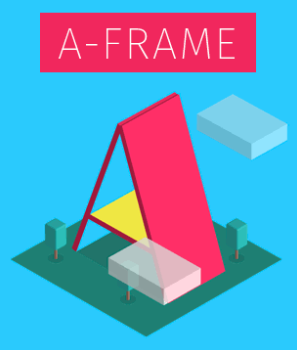
\includegraphics[width=0.25\linewidth]{img/Iconos/Icono_A-Frame.png}
                \caption{Icono de A-Frame}
                \label{fig:otra-imagen}
            \end{minipage}
            \begin{minipage}{0.45\textwidth}
                \centering
                
\includegraphics[width=0.3\linewidth]{img/Iconos/Icono_BabiaXR.png}
                \caption{Icono de BabiaXR}
                \label{fig:html-css-js}
            \end{minipage}\hfill
        \end{figure}
        \subsubsection{A-Frame}
        A-Frame es un framework web para construir experiencias de realidad virtual (VR). A-Frame está basado en HTML, lo que facilita su inicio. Sin embargo, A-Frame no es solo un gráfico de escenas 3D o un lenguaje de marcado; su núcleo es un poderoso framework de entidad-componente que proporciona una estructura declarativa, extensible y componible a three.js.\cite{AFrame}        
        
        A-Frame utiliza Three.js, una popular biblioteca JavaScript para crear gráficos 3D, como motor subyacente para renderizar escenas 3D, lo que permite a los desarrolladores beneficiarse de las características de Three.js, como la gestión avanzada de materiales, luces y sombras, mientras disfrutan de la simplicidad de A-Frame.

        A-Frame también se integra con otras bibliotecas y tecnologías web, como JavaScript y WebGL, permitiendo a los desarrolladores combinar la simplicidad de A-Frame con la complejidad de estas herramientas. Esto hace que A-Frame sea adecuado tanto para proyectos simples como para aplicaciones VR más complejas y avanzadas.

        Otras características, que caben destacar, son las siguientes:
        \begin{itemize}
            \item \textbf{Sintaxis declarativa}: Utiliza una sintaxis similar a HTML para describir escenas 3D.
            \item \textbf{Componentes reutilizables}: Permite la creación de componentes personalizados que pueden ser reutilizados en diferentes partes de la aplicación.
            \item \textbf{Compatibilidad con VR}: Soporta una amplia gama de dispositivos de VR, incluidos Oculus Rift, HTC Vive, y Google Cardboard.
            \item \textbf{Integración con JavaScript}: Permite la interacción y manipulación de escenas mediante JavaScript.
            \item \textbf{Comunidad activa}: Dispone de una amplia biblioteca de ejemplos y componentes creados por la comunidad, facilitando el aprendizaje y la implementación de nuevas funcionalidades.
        \end{itemize}

        Estas son algunas de las áreas a las que va enfocada esta tecnología:

        \begin{itemize}
            \item \textbf{Realidad virtual (VR):} A-Frame facilita la creación de experiencias inmersivas de realidad virtual 
            
            \item \textbf{Realidad aumentada (AR):} Mediante la integración de herramientas y bibliotecas adicionales, A-Frame también soporta el desarrollo de aplicaciones de realidad aumentada.
            
            \item \textbf{Desarrollo web:} A-Frame se basa en HTML y es accesible para desarrolladores web, permitiendo la creación de experiencias 3D y VR directamente en el navegador sin la necesidad de plugins adicionales.
            
            \item \textbf{Educación y entrenamiento:} Debido a su accesibilidad y facilidad de uso, A-Frame es una herramienta popular para la creación de contenidos educativos y de formación.
            
            \item \textbf{Entretenimiento y juegos:} A-Frame permite el desarrollo de juegos y aplicaciones.
            
            \item \textbf{Visualización de datos:} A-Frame puede ser utilizado para la visualización interactiva de datos en 3D.
            
            \item \textbf{Marketing y publicidad:} Las experiencias inmersivas creadas con A-Frame son empleadas en campañas de marketing y publicidad.

        \end{itemize}
        \newpage
        En la siguiente figura (Figura: \ref{fig:Img_Ejemplo_Aframe}) se muestra une ejemplo de escena creada con A-Frame.

        \begin{figure}[H]
            \centering
            \includegraphics[width=0.7\linewidth]{img/Img_Ejemplo_Aframe.png}
            \caption{Ejemplo de escena creada con A-Frame.}
            \label{fig:Img_Ejemplo_Aframe}
        \end{figure}

        
        \subsubsection{BabiaXR}
        BabiaXR es un conjunto de módulos y componentes front-end diseñados para ampliar las capacidades de A-Frame, facilitando la creación de experiencias de realidad extendida (XR). XR es un término que abarca las tecnologías de realidad virtual (VR), realidad aumentada (AR) y realidad mixta (MR). 
        
        
        BabiaXR permite a los desarrolladores crear experiencias interactivas y visualizaciones avanzadas con mayor facilidad, ya que ofrece una colección de herramientas y bibliotecas que simplifican la integración de características avanzadas en aplicaciones A-Frame. Esto incluye componentes específicos para la gestión de interacciones de usuario, efectos visuales avanzados, y soporte para una amplia gama de dispositivos XR. Al proporcionar soluciones listas para usar, BabiaXR reduce significativamente el tiempo y el esfuerzo necesarios para desarrollar aplicaciones XR complejas.
        
        Entre sus características principales se encuentran:
        \begin{itemize}
            \item \textbf{Componentes preconstruidos}: Incluye una variedad de componentes listos para usar.
            \item \textbf{Fácil integración}: Se integra con proyectos A-Frame existentes, lo que facilita la adopción y el uso.
            \item \textbf{Documentación}: Cuenta con documentación y numerosos ejemplos, lo que facilita el aprendizaje y la implementación.
            \item \textbf{Actualizaciones frecuentes}: Mantenido y actualizado regularmente, asegurando que el framework permanezca relevante y compatible con las últimas tecnologías.
        \end{itemize}

        Sus componentes se construyen sobre tecnologías como WebXR, WebGL, A-Frame y Three.js. Entre ellos, se han utilizado los siguientes componentes:

        \begin{itemize}
            \item \textbf{babiaxr-queryjson:} Para consultar datos desde archivos JSON y almacenarlos en una entidad para su posterior visualización.
        
            \item \textbf{babiaxr-selector:} Para seleccionar datos desde una entidad de datos consultados y controlarlos a través de un componente de navegación.
        
            \item \textbf{babiaxr-navigator:} Un componente de navegación que permite desplazarse por diferentes períodos de tiempo o estados de datos.
        
            \item \textbf{babiaxr-3dbarchart:} Para crear gráficos de barras en 3D. Este componente permite especificar datos y ajustar ejes y leyendas.
        
            \item \textbf{babiaxr-filterdata:} Para filtrar los datos consultados y guardados por uno de los componentes querier.
        
            \item \textbf{babiaxr-bubbles:} Para la creación de gráficos de burbujas, permitiendo la visualización de tres dimensiones de datos en un formato interactivo y visualmente atractivo.
        
            \item \textbf{babiaxr-task:} Para la gestión de tareas específicas que pueden incluir elementos multimedia como videos.
            
        \end{itemize}


                En la siguiente figura (Figura: \ref{fig:Img_Ejemplo_Aframe}) se muestra une ejemplo de escena creada con BabiaXR.

        \begin{figure}[H]
            \centering
            \includegraphics[width=0.7\linewidth]{img/Img_BabiaXR.png}
            \caption{Escena creada con A-Frame y componente de BabiaXR.}
            \label{fig:Img_Ejemplo_Aframe}
        \end{figure}

        
    \subsection{HTML, Three.js y JavaScript}
    Para poder desarrollar con A-Frame y BabiaXR es necesario tener conocimientos básicos en HTML, JavaScript y Three.js. 
    

            \begin{figure}[H]
            \centering
            \begin{minipage}{0.45\textwidth}
            \centering
            
\includegraphics[width=0.6\linewidth]{img/Iconos/Icono_Html_Css_JS.png}
            \caption{Iconos de HTML, CSS y JavaScript}
            \label{fig:enter-label}
            \end{minipage}
            \begin{minipage}{0.45\textwidth}
                \centering
                \includegraphics[width=0.2\linewidth]{img/Three.js_Icon.png}
                \caption{Icono de Three.js}
                \label{fig:Three.js_Icon}
            \end{minipage}\hfill
        \end{figure}
        \subsubsection{HTML5}        
        HTML, siglas de \textit{HyperText Markup Language} (Lenguaje de Marcado de Hipertexto), es el lenguaje estándar para la creación de páginas web y aplicaciones web. Fue desarrollado originalmente por Tim Berners-Lee en 1991 y ha evolucionado a lo largo de los años, con su quinta versión, HTML5, introducida en 2014.

        HTML5\cite{HTML5,franganillo2010html5} (HyperText Markup Language, versión 5) especifica dos variantes de sintaxis para HTML: una «clásica», HTML (text/html), y una variante XHTML conocida como sintaxis XHTML5 que deberá servirse con sintaxis XML (application/xhtml+xml).\cite{HTML5}


        Entre sus características principales se encuentran:
        \begin{itemize}
            \item \textbf{Lenguaje de Marcado}: HTML utiliza etiquetas (\textit{tags}) para describir la estructura y el contenido de una página web.
            \item \textbf{Secciones}: Permite organizar el contenido en secciones como encabezados, párrafos, listas, tablas, enlaces, imágenes y formularios.
            \item \textbf{Compatibilidad}: Es compatible con una amplia gama de navegadores y dispositivos, asegurando que el contenido sea accesible para todos los usuarios.
            \item \textbf{Integración con otros lenguajes}: HTML puede ser combinado con CSS (Cascading Style Sheets) para el diseño y con JavaScript para la interactividad.
        \end{itemize}

        Estas son algunas de las características introducidas en la última versión de HTML5, que han facilitado el desarrollo e implementación de las nuevas tecnologías.

        \begin{itemize}
            \item \textbf{Nuevos elementos semánticos}: Introduce elementos como \texttt{<header>}, \texttt{<footer>}, \texttt{<article>} y \texttt{<section>}, mejorando la semántica y accesibilidad del contenido web.
            \item \textbf{Soporte multimedia}: Incorpora elementos \texttt{<audio>} y \texttt{<video>} para la integración directa de contenido multimedia sin necesidad de plugins adicionales.
            \item \textbf{Gráficos y animaciones}: El elemento \texttt{<canvas>} y la integración de SVG permiten la creación de gráficos y animaciones dinámicas.
            \item \textbf{Almacenamiento local}: Proporciona APIs como \texttt{localStorage} y \texttt{sessionStorage} para almacenar datos en el navegador del usuario.
            \item \textbf{Formularios mejorados}: Nuevos tipos de \texttt{input} y atributos que facilitan la validación y el control de datos en formularios.
        \end{itemize}
        
        
        \subsubsection{JavaScript}
        JavaScript\cite{JavaScriptMDN,ECMAScript,JavaScriptWikibooks} es un lenguaje de programación de alto nivel, interpretado y orientado a objetos, creado por Brendan Eich en 1995.

        Es un lenguaje de programación ligero, interpretado, o compilado justo-a-tiempo (just-in-time) con funciones de primera clase. Si bien es más conocido como un lenguaje de scripting (secuencias de comandos) para páginas web, y es usado en muchos entornos fuera del navegador, tal como Node.js, Apache CouchDB y Adobe Acrobat. JavaScript es un lenguaje de programación basado en prototipos, multiparadigma, de un solo hilo, dinámico, con soporte para programación orientada a objetos, imperativa y declarativa (por ejemplo, programación funcional).


        Entre sus características principales se encuentran:
        \begin{itemize}
            \item \textbf{Lenguaje interpretado}: Se ejecuta directamente en el navegador del usuario sin necesidad de compilación previa.
            \item \textbf{Manipulación del DOM}: Permite interactuar y manipular los elementos del Documento de Modelo de Objetos (DOM) de una página web, lo que facilita la actualización dinámica del contenido.
            \item \textbf{Eventos y funciones}: Gestión de eventos del usuario (como clics, desplazamientos y entradas de teclado) y ejecución de funciones en respuesta a esos eventos.
            \item \textbf{Asincronía}: Soporte para operaciones asincrónicas mediante callbacks, promesas y la sintaxis \texttt{async/await}, lo que permite manejar tareas concurrentes sin bloquear la ejecución del código.
            \item \textbf{APIs Integradas}: Acceso a una variedad de APIs del navegador, como geolocalización, almacenamiento local y la API \texttt{fetch} para realizar solicitudes HTTP.
        \end{itemize}

        \subsubsection{Three.js}
        Three.js\cite{ThreeJS,dirksen2013learning,} es una biblioteca JavaScript multiplataforma y una interfaz de programación de aplicaciones (API).
        
        Three.js permite la creación de animaciones 3D aceleradas por la unidad de procesamiento gráfico (GPU), utilizando el lenguaje JavaScript como parte de un sitio web sin depender de complementos propietarios del navegador. Esto es posible gracias al surgimiento de WebGL, una API gráfica de bajo nivel creada específicamente para la web.\cite{ThreeJS}
        
        Entre sus características principales se encuentran:

    \begin{itemize} 
        \item \textbf{Geometrías y materiales:} Soporta una gran variedad de formas geométricas y diversos materiales básicos.    
        \item \textbf{Iluminación y sombras:} Cuenta con diferentes tipos de luces: puntuales, direccionales, ambientales, y con la creación de sombras realistas.    
        \item \textbf{Texturas:} Aplicación de texturas a objetos.Soporte para mapas de normales, mapas de desplazamiento y mapas ambientales.    
        \item \textbf{Animaciones:} Herramientas para animar objetos, cámaras, animaciones esqueléticas y de personajes.    
        \item \textbf{Compatibilidad y extensibilidad:} Funciona en la mayoría de los navegadores modernos y dispositivos móviles. Extensible con plugins personalizados y fácil integración con otras bibliotecas.    
        \item \textbf{Comunidad y recursos:} Cuenta con una extensa documentación y numerosos ejemplos.
    \end{itemize}

  

    \subsection{Python y Flask}
        \begin{figure}[H]
            \centering
            \begin{minipage}{0.45\textwidth}
                \centering
                
\includegraphics[width=0.25\linewidth]{img/Iconos/Icono_Python.png}
                \caption{Icono de Python}
                \label{fig:otra-imagen}
            \end{minipage}
            \begin{minipage}{0.45\textwidth}
                \centering
                
\includegraphics[width=0.26\linewidth]{img/Iconos/Icono_Flask.png}
                \caption{Icono de Flask}
                \label{fig:html-css-js}
            \end{minipage}\hfill
        \end{figure}

        \subsubsection{Python}
        Python\cite{PythonWikibooks,knowltonPython} es un lenguaje de programación de alto nivel, creado por Guido van Rossum y lanzado por primera vez en 1991. Python es conocido por su sintaxis clara y legible, lo que facilita la escritura y el mantenimiento del código. Es ampliamente utilizado en diversas áreas de la informática, desde el desarrollo web hasta la ciencia de datos y la inteligencia artificial.
        
        Entre sus características principales se encuentran:

        \begin{itemize}
            \item \textbf{Sintaxis clara y legible}: Python está diseñado para ser fácil de leer y escribir, lo que mejora la productividad del desarrollador.
            \item \textbf{Versatilidad}: Es un lenguaje utilizado en una amplia variedad de aplicaciones como desarrollo web, automatización, análisis de datos, inteligencia artificial, entre otros.
            \item \textbf{Bibliotecas extensas}: Python cuenta con una vasta colección de bibliotecas y frameworks que facilitan el desarrollo en diferentes dominios, como Django y Flask para el desarrollo web, Pandas y NumPy para el análisis de datos, y TensorFlow y PyTorch para el aprendizaje automático.
            \item \textbf{Interpretable}: Python se ejecuta en tiempo de ejecución, lo que permite la ejecución interactiva de código y facilita la depuración.
        \end{itemize}

        Python\cite{PythonWikibooks,PythonTutorial} está diseñado para ser utilizado en diversas áreas, incluyendo:
        \begin{itemize}
            \item \textbf{Desarrollo web}: Creación de aplicaciones web utilizando frameworks como Django y Flask.
            \item \textbf{Ciencia de datos}: Análisis de datos, visualización y machine learning utilizando bibliotecas como Pandas, NumPy, Matplotlib, y Scikit-learn.
            \item \textbf{Automatización}: Automatización de tareas repetitivas y escritura de scripts.
            \item \textbf{Inteligencia artificial}: Desarrollo de modelos de inteligencia artificial y aprendizaje profundo utilizando frameworks como TensorFlow y PyTorch.
            \item \textbf{Desarrollo de software}: Uso en el desarrollo de aplicaciones de escritorio, juegos y otros tipos de software.
        \end{itemize}
        
        \subsubsection{Flask}
        Flask es un microframework de desarrollo web para Python, creado por Armin Ronacher y lanzado en 2010. 
        
        Entre sus características principales se encuentran:
\begin{itemize}
    \item{Integración Sencilla con el Desarrollo Web}: Flask es un microframework de desarrollo web para Python que facilita la creación de aplicaciones web. Al usar Flask, puedes:
        \begin{itemize}
            \item Crear fácilmente rutas HTTP que pueden ser accedidas desde el frontend mediante solicitudes AJAX.
            \item Integrar lógica de backend escrita en Python con la interfaz de usuario de tu aplicación web.
        \end{itemize}

    \item{Manejo de Solicitudes HTTP}: Flask proporciona herramientas integradas para manejar solicitudes HTTP, lo cual es esencial cuando se interactúa con el DOM. Con Flask, puedes:
        \begin{itemize}
            \item Definir rutas para manejar diferentes tipos de solicitudes (GET, POST, PUT, DELETE).
            \item Procesar datos enviados desde el frontend y devolver respuestas adecuadas en formato JSON, HTML, etc.
        \end{itemize}

    \item \textbf{Aplicaciones microservicio}: Implementación de servicios pequeños y modulares.
    \item \textbf{Aplicaciones de escritorio}: Uso en la creación de interfaces gráficas para aplicaciones de escritorio mediante herramientas como Flask-Electron.
\end{itemize}
        
\section{Herramientas de desarrollo} 
\label{sec:Herramientas}
En este apartado se describirán las principales herramientas tecnológicas empleadas, destacando cómo cada una contribuye al desarrollo del proyecto.

    \subsection{Desarrollo y gestión de código} 
    
    Para el entorno de desarrollo y la gestión de código, se han seleccionado dos herramientas que ofrecen facilidad de uso y eficiencia: Visual Studio Code y GitHub.
    
    
    \begin{figure}[H]
        \centering
        
\includegraphics[width=0.1\linewidth]{img/Iconos/Icono_VS_Code.png}
        \caption{Visual Studio Code: Icono}
        \label{fig:enter-label}
    \end{figure}
    
    \subsubsection{Visual Studio Code}
    
    Visual Studio Code (VS Code) es un editor de código fuente desarrollado por Microsoft, lanzado por primera vez en abril de 2015. Es una herramienta que soporta una amplia gama de lenguajes de programación y tecnologías. Algunas de sus características más destacadas incluyen:
    \begin{itemize}
        \item\textbf{Multiplataforma:} Está disponible para Windows, macOS y Linux, lo que permite a los desarrolladores trabajar en cualquier sistema operativo.
        \item\textbf{Extensiones:} Cuenta con la opción de miles de extensiones en el marketplace, que permiten añadir nuevas funcionalidades, soporte para distintos lenguajes de programación, integraciones con herramientas de desarrollo y personalización del entorno de trabajo.
        \item\textbf{Depuración:} VS Code incluye potentes herramientas de depuración que permiten a los desarrolladores encontrar y corregir errores en su código de manera fácil.
        \item\textbf{Control de versiones:} La integración con sistemas de control de versiones como Git está incorporada de forma nativa, facilitando la gestión del código fuente y la colaboración en proyectos.
        \item\textbf{Terminal integrada:} La terminal integrada permite ejecutar comandos directamente desde el editor, sin necesidad de cambiar de ventana o aplicación.
        \item\textbf{IntelliSense:} Esta característica ofrece autocompletado inteligente y sugerencias de código basadas en el contexto y la sintaxis del lenguaje de programación utilizado.
    \end{itemize}
    
    En comparación con otros editores de código, VS Code se destaca por su velocidad, la riqueza de su ecosistema de extensiones y su integración sin problemas con herramientas de desarrollo populares. Además, su interfaz amigable hace que sea una opción ideal tanto para desarrolladores principiantes como para avanzados. Más información sobre Visual Studio Code está disponible en Visual Studio Code.
    
    \vspace{0.5cm} % Inserta un espacio vertical de 0.5 cm
    \textbf{Aplicación en el proyecto:} 
    
    Visual Studio Code ha sido utilizado como entorno de desarrollo para todos los componentes necesarios, así como para la ejecución y depuración del código. Para poder llevar a cabo todo ello, se implemento una de sus extensiones.
    
    \begin{itemize}   
        \begin{figure}[H]
            \centering
            
\includegraphics[width=0.1\linewidth]{img/Iconos/Icono_Live_Server.png}
            \caption{Live Server: Icono}
            \label{fig:enter-label}
        \end{figure}
        \item \textbf{Extensión Live Server:} Live Server ha sido desarrollada por Ritwick Dey. Esta extensión permite lanzar un servidor local de desarrollo con funcionalidad de recarga en vivo para páginas estáticas y dinámicas, permitiendo una retroalimentación instantánea. La extensión Live Server se distribuye bajo la licencia MIT, que permite un uso amplio y flexible del software, garantizando que se incluya un aviso de copyright y la licencia. El código de Live Server está disponible en su repositorio de GitHub\footnote{\url{https://github.com/ritwickdey/vscode-live-server}}.  
    \end{itemize}
    
    
    \subsubsection{GIT y GitHub:}
        \begin{figure}[H]
            \centering
            
\includegraphics[width=0.1\linewidth]{img/Iconos/Icono_Git.png}
            \caption{Git: Icono}
            \label{fig:enter-label}
         \end{figure}
        
        \textbf{Git:} Es un sistema de control de versiones distribuido, desarrollado por Linus Torvalds en 2005. Es una herramienta que permite a los desarrolladores rastrear y gestionar cambios en el código fuente a lo largo del tiempo. Algunas de sus características más destacadas incluyen:
    
        \begin{itemize}
            \item \textbf{Control de versiones distribuido}: A diferencia de los sistemas, cada clon de un repositorio Git es un repositorio completo con historial completo.
            \item \textbf{Eficiencia y rapidez}: Git permite realizar operaciones como commits, branches, merges y comparaciones de manera muy rápida.
            \item \textbf{Integridad de los datos}: Cada cambio en el código es rastreado y registrado de forma segura, utilizando una técnica de hash criptográfico (SHA-1), lo que garantiza la integridad y autenticidad de los datos.
            \item \textbf{Branching y merging}: Git facilita la creación y manejo de ramas (branches), permitiendo a los desarrolladores trabajar de forma simultánea. Las ramas pueden fusionarse cuando sea necesario.
        \end{itemize}
    
        \begin{figure}[H]
            \centering
            
\includegraphics[width=0.1\linewidth]{img/Iconos/Icono_GitHub.png}
            \caption{GitHub: Icono}
            \label{fig:enter-label}
         \end{figure}
        
        \textbf{GitHub} es una plataforma de alojamiento de código fuente y gestión de proyectos basada en Git, creada en 2008. Ofrece una variedad de herramientas y características para facilitar la colaboración y el desarrollo de software. Algunas de sus funcionalidades clave incluyen:
    
        \begin{itemize}
            \item \textbf{Repositorios}: GitHub permite almacenar repositorios Git en la nube.
            \item \textbf{Colaboración}: A través de pull requests, issues y discusiones, los desarrolladores pueden colaborar de manera efectiva, revisando cambios y sugiriendo mejoras.
            \item \textbf{Integración continua}: GitHub se integra con diversas herramientas de CI/CD, permitiendo la automatización de pruebas, despliegues y otras tareas de desarrollo.
            \item \textbf{Páginas de GitHub}: Permite a los usuarios hospedar sitios web estáticos directamente desde sus repositorios.
            \item \textbf{Seguridad y gestión}: GitHub proporciona herramientas para la revisión de código, gestión de dependencias y seguridad, ayudando a mantener la calidad y seguridad del software.
            \item \textbf{Marketplace y aplicaciones}: Ofrece una amplia gama de aplicaciones y herramientas adicionales a través de su marketplace.
        \end{itemize}
    
        Git y GitHub se utilizan conjuntamente en la mayoría de los proyectos de software modernos. Git se encarga del control de versiones a nivel local, mientras que GitHub ofrece una plataforma para almacenar y compartir repositorios, facilitando la colaboración y el despliegue de proyectos. 
        
        \vspace{0.5cm} % Inserta un espacio vertical de 0.5 cm
        \textbf{Aplicación en el proyecto:} 
        
       Git y GitHub se han utilizado para el control de versiones y el almacenamiento del repositorio, garantizando la seguridad mediante copias de respaldo. Estas herramientas permiten hospedar el proyecto y compartir el código fácilmente. Además, han sido empleadas para clonar otros repositorios necesarios para el desarrollo del proyecto, como BabiaXR\footnote{\url{https://github.com/babiaxr/aframe-babia-components}} y la plantilla de la memoria\footnote{\url{https://github.com/gregoriorobles/plantilla-memoria.}}
        
    
    
    
    
    
    \subsection{Creación y edición de contenidos visuales y multimedia}
    
    Para la creación de contenidos audiovisuales y multimedia, se han utilizado diversas herramientas como Animaker, Canva y SpeechGen, con el objetivo de minimizar la necesidad de gestionar derechos de autor.
    
        \begin{figure}[H]
            \centering
            
\includegraphics[width=0.3\linewidth]{img/Iconos/Icono_Animaker.png}
            \caption{Animaker: Icono}
            \label{fig:enter-label}
         \end{figure}     
        \subsubsection{Animaker}
    
    Animaker es una plataforma, lanzada en 2014, de creación de vídeos animados que permite a los usuarios diseñar y producir contenido visual sin necesidad de conocimientos avanzados en animación. Animaker ofrece una variedad de herramientas y recursos que facilitan la creación de vídeos para diferentes propósitos, como presentaciones, marketing, educación y entretenimiento.
    
    Algunas de sus características principales son:
    
    \begin{itemize}
        \item \textbf{Interfaz intuitiva}: Cuenta con una interfaz fácil de usar basada en el método de arrastrar y soltar (\textit{drag-and-drop}), lo que permite crear vídeos rápidamente sin necesidad de tener habilidades técnicas avanzadas.
        \item \textbf{Biblioteca de recursos}: La plataforma ofrece una extensa biblioteca de recursos, incluyendo personajes, íconos, fondos, y efectos de sonido.
        \item \textbf{Plantillas predefinidas}: Animaker proporciona una amplia gama de plantillas predefinidas que cubren diversos tipos de vídeos.
        \item \textbf{Animaciones personalizadas}: Los usuarios pueden crear animaciones personalizadas utilizando herramientas que permiten ajustar movimientos, expresiones faciales y acciones de los personajes.
        \item \textbf{Text-to-Speech y Voiceover}: La plataforma incluye funciones de conversión de texto a voz y grabación de voz en off, lo que permite añadir narraciones personalizadas a los videos.
        \item \textbf{Exportación}: Permite exportar vídeos en varias resoluciones y formatos. Además, los vídeos pueden ser compartidos directamente desde la plataforma.
        \item \textbf{Colaboración en tiempo real}: Para equipos de trabajo, permite a varios usuarios trabajar en el mismo proyecto simultáneamente.
    \end{itemize}
    
        \vspace{0.5cm} % Inserta un espacio vertical de 0.5 cm
        \textbf{Aplicación en el proyecto:} 
        
       Animaker\footnote{\url{https://www.animaker.com/}} se ha empleado para crear los contenidos audiovisuales utilizados en la representación de datos.
    
    
        \begin{figure}[H]
            \centering
            
\includegraphics[width=0.1\linewidth]{img/Iconos/Icono_Canva.png}
            \caption{Canva: Icono}
            \label{fig:enter-label}
         \end{figure}
        \subsubsection{Canva}
    
        Canva es una plataforma de diseño gráfico en línea, fundada en 2012, que permite a los usuarios crear gráficos, presentaciones, carteles y otros contenidos visuales.
        
        Algunas de sus características principales son:
    
        \begin{itemize}
            \item Tiene una interfaz muy intuitiva.
            \item Cuenta con una extensa biblioteca de recursos.
            \item Contiene plantillas predefinidas.
            \item Permite exportar en PNG, JPG, PDF y MP4, y compartir fácilmente en redes sociales, sitios web y presentaciones.
            \item Cuenta con colaboración en Tiempo Real.
        \end{itemize}
    
        \vspace{0.5cm} % Inserta un espacio vertical de 0.5 cm
        \textbf{Aplicación en el proyecto:} 
        
        Canva\footnote{\url{https://www.canva.com/}} se ha utilizado para diseñar las imágenes que acompañan la documentación.
    
    
    
    
    
    
    \subsection{Documentación}  
    Para la creación de la documentación del proyecto, se ha utilizado LaTeX, una herramienta enfocada en la composición de textos científicos y técnicos.
    
        \begin{figure}[H]
            \centering
            
\includegraphics[width=0.15\linewidth]{img/Iconos/Icono_Latex.png}
            \caption{LaTeX: Icono}
            \label{fig:enter-label}
         \end{figure}
    \subsubsection{LaTeX}
    
        LaTeX\cite{sanguino1997iniciacion} es un sistema de preparación de documentos de alta calidad desarrollado por Leslie Lamport en la década de 1980 sobre el sistema de tipografía TeX, creado por Donald Knuth. 
        
        Algunas de sus características principales son:
    
        \begin{itemize}
            \item \textbf{Alta calidad tipográfica}: LaTeX es conocido por producir documentos con una excelente calidad tipográfica, lo que lo hace ideal para la publicación de trabajos académicos, artículos científicos, tesis y libros.
            \item \textbf{Separación de contenido y formato}: LaTeX permite a los usuarios concentrarse en el contenido del documento, dejando el formato y la presentación a los comandos de LaTeX. Esto garantiza una consistencia en el diseño del documento.
            \item \textbf{Manejo de referencias y bibliografía}: LaTeX incluye herramientas avanzadas para la gestión de referencias cruzadas, citas y bibliografías, facilitando la creación de documentos académicos con referencias complejas.
            \item \textbf{Soporte para fórmulas matemáticas}: LaTeX es ampliamente utilizado en campos científicos y matemáticos debido a su capacidad para representar fórmulas y ecuaciones de manera clara y precisa.
            \item \textbf{Extensibilidad}: LaTeX es altamente extensible a través de paquetes adicionales que pueden añadirse para proporcionar nuevas funcionalidades, como gráficos, tablas avanzadas y diagramas.
            \item \textbf{Documentos estructurados}: LaTeX permite crear documentos bien estructurados con secciones, subsecciones, tablas de contenido, índices y listas de figuras y tablas.
        \end{itemize}
    
    \textbf{Ventajas}
    
    \begin{itemize}
        \item {Asegura que el formato del documento se mantenga consistente a lo largo del texto.}
        \item {Cuenta con una extensa comunidad de usuarios y desarrolladores, así como una gran cantidad de documentación y recursos en línea.}
        \item {Es gratuito y de código abierto}
    \end{itemize}
    
    \textbf{Desventajas}
    
    \begin{itemize}
        \item {LaTeX puede ser difícil de aprender para principiantes debido a su sintaxis basada en comandos.}
        \item {La configuración inicial de un documento puede ser compleja, especialmente para documentos grandes.}
    \end{itemize}
    
        \vspace{0.5cm} % Inserta un espacio vertical de 0.5 cm
        \textbf{Aplicación en el proyecto:} 
        
        LaTeX\footnote{\url{https://www.latex-project.org/}} se ha utilizado para elaborar la documentación del proyecto, buscando una alta calidad.
    
    
    







    


\section{Fuentes de recursos} 
\label{sec:Recursos}
En este apartado se nombra y explica las fuente de recursos que utiliza el proyecto para mostrar la funcionalidad de los diferentes elementos.

    \subsection{Fuente de Datos} 
        \begin{figure}[H]
            \centering
            
\includegraphics[width=0.3\linewidth]{img/Iconos/Icono_Eurostat.png}
            \caption{Eurostat: Icono}
            \label{fig:enter-label}
         \end{figure}
    
    Los datos representados en este proyecto provienen de la base de datos de Eurostat\footnote{\url{https://ec.europa.eu/eurostat/databrowser/view/sdg_13_10/default/table?lang=en}}. Esta es la oficina estadística de la Unión Europea, responsable de proporcionar estadísticas a nivel europeo. Su misión es ofrecer datos de alta calidad y comparables sobre una amplia gama de temas para apoyar la toma de decisiones, la investigación y el análisis a nivel europeo.
    
    Eurostat recopila datos de los institutos nacionales de estadística de los Estados miembros y de otros países europeos, procesándolos y armonizándolos para garantizar su comparabilidad. Las áreas de interés incluyen economía, medio ambiente, salud, educación, y muchos otros aspectos sociales y demográficos.
    
    Para este proyecto, se seleccionaron los datos referentes a las emisiones de CO2 en línea con el Objetivo de Desarrollo Sostenible (ODS) 13\footnote{\url{https://ec.europa.eu/eurostat/en/}}.
    
    \subsection{Imágenes} 
    \begin{itemize}
        \item \textbf{Freepik}: Freepik es una plataforma en línea fundada en 2010 que proporciona recursos gráficos gratuitos para diseñadores y desarrolladores.
        Muchas de las imágenes utilizadas para la texturización del entorno se han obtenido en Freepik.
        \item \textbf{Canva}: Canva se ha utilizado para crear y editar imágenes personalizadas para la documentación del proyecto. Los detalles sobre la herramienta se explican en profundidad en el apartado de herramientas de desarrollo (ver Sección \ref{sec:Herramientas}).
    \end{itemize}
    
    \subsection{Vídeos}
    \begin{itemize}
        \item \textbf{Animaker}: Animaker a parte de ser utilizado para crear y editar audios y animaciones, es la fuente de donde se han obtenido los vídeos base. Los detalles sobre la herramienta se explican en profundidad en el apartado de herramientas de desarrollo (ver Sección \ref{sec:Herramientas}).
    \end{itemize}
    
    \subsection{Audios} 
    \begin{itemize}
        \item \textbf{SpeechGen}: SpeechGen\footnote{\url{https://speechgen.io/es/}{SpeechGen}} es una herramienta avanzada de conversión de texto a voz (TTS) impulsada por inteligencia artificial. Con esta herramienta se han generado todos los audios de la visualización.
    \end{itemize}
    \subsection{Objetos 3D} 
    \begin{itemize}
        \item \textbf{Sketchfab}: Sketchfab\footnote{\url{https://sketchfab.com/}{Sketchfab}} es una plataforma para la visualización y la publicación de modelos 3D en la web. Ofrece herramientas para que los usuarios puedan mostrar y compartir contenido 3D de manera interactiva, directamente desde el navegador, sin necesidad de instalar software adicional.
    \end{itemize}
    

%%%%%%%%%%%%%%%%%%%%%%%%%%%%%%%%%%%%%%%%%%%%%%%%%%%%%%%%%%%%%%%%%%%%%%%%%%%%%%%%
%%%%%%%%%%%%%%%%%%%%%%%%%%%%%%%%%%%%%%%%%%%%%%%%%%%%%%%%%%%%%%%%%%%%%%%%%%%%%%%%
% DISEÑO E IMPLEMENTACIÓN %
%%%%%%%%%%%%%%%%%%%%%%%%%%%%%%%%%%%%%%%%%%%%%%%%%%%%%%%%%%%%%%%%%%%%%%%%%%%%%%%%

\cleardoublepage

\section{Otros}

La planificación y desarrollo del proyecto se inspiró en la metodología Ágil Scrum.

\subsection{Scrum}
Scrum es un marco de trabajo ágil que surgió en la década de 1990, basado en principios de desarrollo iterativo e incremental, con el fin de gestionar y desarrollar proyectos, principalmente en el campo del software. Scrum se organiza en ciclos cortos y repetitivos llamados 'sprints', que generalmente duran de una a cuatro semanas. Cada sprint incluye fases de planificación, ejecución, revisión y retrospectiva, lo que permite adaptarse rápidamente a los cambios y mejorar continuamente. Este enfoque fomenta la colaboración del equipo, la entrega frecuente de productos funcionales, la integración del feedback de los usuarios y el aumento de la calidad del producto final.


Los elementos clave de Scrum incluyen los roles, eventos y artefactos, cada uno desempeñando un papel crucial en el proceso de desarrollo ágil.

\subsubsection{Roles}
Scrum define tres roles principales:

\begin{itemize}
    \item \textbf{Product Owner}: Responsable de maximizar el valor del producto y gestionar el Product Backlog. El Product Owner se asegura de que el equipo trabaje en las tareas correctas desde una perspectiva del negocio.
    \item \textbf{Scrum Master}: Facilita el proceso Scrum y elimina impedimentos para el equipo. El Scrum Master actúa como un coach para el equipo y el Product Owner, asegurando que se sigan las prácticas Scrum.
    \item \textbf{Development Team}: Un equipo autoorganizado y multifuncional que trabaja en los incrementos del producto. El equipo de desarrollo es responsable de la entrega de funcionalidades potencialmente liberables al final de cada sprint.
\end{itemize}

\begin{figure}[H]
  \centering
  \includegraphics[width=11cm, keepaspectratio]{img/Scrum_roles.png}
  \caption{Scrum: Roles}
  \label{fig:roles}
\end{figure}


\subsubsection{Eventos}
Scrum utiliza una serie de eventos para crear regularidad y minimizar la necesidad de reuniones:

\begin{itemize}
    \item \textbf{Sprint}: Un ciclo de trabajo de tiempo fijo (generalmente de 2 a 4 semanas) durante el cual se crea un incremento del producto.
    \item \textbf{Sprint Planning}: Una reunión al inicio del sprint donde el equipo define qué se hará durante el sprint y cómo se logrará.
    \item \textbf{Daily Scrum}: Reuniones diarias de 15 minutos donde el equipo sincroniza actividades y planifica el trabajo de las próximas 24 horas.
    \item \textbf{Sprint Review}: Una reunión al final del sprint donde el equipo presenta lo que se ha completado durante el sprint a los stakeholders y recoge feedback.
    \item \textbf{Sprint Retrospective}: Una reunión después del Sprint Review donde el equipo reflexiona sobre el sprint pasado y planifica mejoras para el siguiente.
\end{itemize}



\subsubsection{Artefactos}

Scrum utiliza tres artefactos principales para gestionar el trabajo:

\begin{itemize}
    \item \textbf{Product Backlog}: Una lista ordenada de todo lo que podría ser necesario en el producto, gestionada por el Product Owner.
    \item \textbf{Sprint Backlog}: El conjunto de elementos del Product Backlog seleccionados para el sprint, junto con un plan para entregarlos.
    \item \textbf{Increment}: La suma de todos los elementos del Product Backlog completados durante un sprint y todos los sprints anteriores. El incremento debe estar en un estado utilizable y cumplir con la definición de "Terminado".
\end{itemize}

\begin{figure}[H]
  \centering
  \includegraphics[width=12cm, keepaspectratio]{img/Scrum_Eventos_Artefactos.png}
  \caption{Scrum: Roles, Eventos y Artefactos}
  \label{fig:roles}
\end{figure}



\chapter{Desarrollo del proyecto}
\label{sec:Desarrollo}

En este capítulo se describirá la conceptualización, el planteamiento y el seguimiento del proyecto, desde su inicio hasta la finalización de todas las tareas especificadas. Primero, se ofrecerá una visión general del planteamiento del desarrollo, mencionando la metodología utilizada y el entorno de trabajo empleado. Posteriormente, se presentará cada etapa del desarrollo, explicando su objetivo, estructura en detalle y tecnologías empleadas para su implementación.

\section{Visión General} 

Normalmente, los proyectos comienzan con una estrategia que guía su desarrollo y seguimiento. En esta ocasión, para plantear esta fase inicial, se eligió una metodología de trabajo inspirada en los principios de la metodología ágil conocida como Scrum.

Scrum es una metodología ágil de gestión de proyectos utilizada principalmente en el desarrollo de software. Se enfoca en la entrega incremental y iterativa de productos, permitiendo adaptarse rápidamente a los cambios y mejorar continuamente. Esta metodología se explica con mas detalle en el apartado \ref{chap:tecnologías}.

Al no contar con los elementos necesarios para utilizar completamente la metodología Scrum, se realizó una adaptación seleccionando los elementos más beneficiosos para el desarrollo del proyecto. En particular, se adoptó la práctica de dividir el proyecto en tareas más pequeñas, según la necesidades que vayan surgiendo, y agruparlas en Sprints. Esto permitió una mejor organización y seguimiento del progreso del proyecto. Además, al trabajar en Sprints, se logró un desarrollo incremental que permitió ajustes basados en la retroalimentación constante.

A continuación se detallan los sprints realizados durante el proyecto. Cada sprint representa una iteración del ciclo de desarrollo, en la que se han abordado diferentes tareas y objetivos.

\section{Sprint 0}
El Sprint 0 suele ser la etapa inicial de un proyecto en la que se establecen las bases necesarias para los siguientes sprints. En esta fase, se configuró el entorno de desarrollo, se identifico los requisitos iniciales y se prepararon las herramientas y recursos necesarios para los siguientes sprints.

A continuación se detallaran las especificaciones y tareas que se desarrollaron en este sprint:

        \begin{itemize}
            \item \textbf{Especificaciones:}
            \begin{itemize}
                \item \textbf{Objetivo:} Establecer las bases del proyecto y preparar el entorno de desarrollo.
                \item \textbf{Duración:} 1 semanas.
            \end{itemize}
            
            \item \textbf{Tareas:}
            \begin{enumerate}
                \item Identificar y planificar los requisitos iniciales, en tareas, para los primeros Sprints.
                \item Preparar las herramientas y recursos necesarios.
            \end{enumerate}
        \end{itemize}

    \subsection{Identificar y documentar los requisitos iniciales:}

    El análisis inicial de los requisitos reveló que, debido a la diversidad de lenguajes y tecnologías involucradas, sería conveniente dividir la fase de aprendizaje en dos sprints: Sprint 1 y Sprint 2. El primer sprint se centraría en establecer las bases necesarias para crear una escena básica y funcional en realidad virtual. El segundo sprint se enfocaría en adquirir los conocimientos necesarios para integrar componentes ya desarrollados, como BabiaXR, que permitan mostrar los datos mediante gráficos dentro de la escena virtual.

    Los conocimientos básicos que se detectaron como necesarios para crear una escena en realidad virtual fueron los siguientes:
    \begin{itemize} 
        \item \textbf{Conocimientos básicos de A-Frame:} Es esencial para estructurar y definir la escena 3D.
        \item \textbf{Conocimientos básicos de Three.js:} Proporciona las herramientas necesarias para construir geometrías, materiales y animaciones complejas.    
        \item \textbf{Conocimientos básicos de JavaScript:} El lenguaje fundamental para la manipulación y control de los elementos en la escena, incluyendo la lógica de interacción y la integración con otras bibliotecas como A-Frame y Three.js.   
    \end{itemize}

    En cambio, para mostrar datos mediante gráficos, se identificaron los siguientes conocimientos como necesarios:
    \begin{itemize}
        \item \textbf{Conocimientos de BabiaXR:} Esta plataforma facilita la visualización de datos en entornos de realidad extendida.
        \item \textbf{Conocimientos de visualización de datos y gráficos:} Comprender cómo representar datos de manera efectiva, utilizando gráficos adecuados para cada tipo de información.
    \end{itemize}

    En la siguiente figura (Figura: \ref{fig:ImgS0}), se muestra como se hizo la distribución de las tareas:
\begin{figure}[h]
    \centering
    \includegraphics[width=0.5\linewidth]{img/ImgS0.png}
    \caption{Sprint 0: Distribución de tareas iniciales}
    \label{fig:ImgS0}
\end{figure}
    
\vspace{1em}
    \subsection{Herramientas y recursos necesarios.}
    
    Para la elaboración del proyecto se preparo un entorno de trabajo con las siguientes herramientas:
        
    \begin{itemize}
        \item \textbf{Windows como sistema operativo:} Ha sido elegido, por su amplia compatibilidad, facilidad de uso y soporte de software.   
        \item \textbf{Chrome y Firefox como navegadores:} Utilizados para la realización de pruebas y depuración, debido a su compatibilidad con estándares web y sus avanzadas herramientas para desarrolladores.   
        \item \textbf{Visual Studio Code como entorno de desarrollo:} Ha sido elegido por su facilidad de uso, soporte para múltiples lenguajes de programación y una amplia gama de extensiones que mejoran el desarrollo, control y depuración del código. Se instalo adicionalmente la extensión Live Server para la ejecución en tiempo real. 
        \item \textbf{GitHub como control de versiones:} Se ha utilizado para gestionar el código fuente, proporcionando un punto de control y seguridad. Además, GitHub Pages proporcionó una forma sencilla de ejecutar el código directamente desde el repositorio.   
    \end{itemize}


    
    
    \newpage
    \section{Sprint 1}

    En el primer sprint, el objetivo principal es adquirir los conocimientos básicos y habilidades necesarias para crear una escena en realidad virtual. Este sprint se centro en el aprendizaje de tecnologías fundamentales y en la creación de una escena funcional.

    A continuación se detallan las especificaciones y tareas establecidas para este sprint:
        \begin{itemize}
            \item \textbf{Especificaciones:}
            \begin{itemize}
                \item \textbf{Objetivo:} Crear escenas funcionales y agradables en VR.
                \item \textbf{Duración:} 3 semanas.
            \end{itemize}
            
            \item \textbf{Tareas:}
            \begin{enumerate}
                \item Obtener conocimientos en A-Frame.
                \item Revisar y actualizar conocimientos en Three.js.
                \item Revisar y actualizar conocimientos en JavaScript.
            \end{enumerate}

            Todas estas tareas se llevaron a cabo recopilando conocimientos a través de apuntes, tutoriales en línea, documentación oficial y realización de prácticas.

            A la hora de realizar las prácticas, se crearon escenarios de prueba donde se desarrollaban componentes básicos y se experimentaba con diferentes funcionalidades. Estos escenarios permitieron entender mejor cómo interactuar con las tecnologías involucradas y resolver problemas comunes.
           \end{itemize} 

            \subsection{Prototipos:}

            Durante el aprendizaje de los conceptos básicos, se realizaron ejercicios prácticos para aplicar los conocimientos adquiridos. El último ejercicio, dio como resultado la escena que se puede apreciar en la Figura  \ref{fig:Prototipo1}.

            En esta escena se han utilizado HTML, A-Frame, Three.js y JavaScript. Se han empleado figuras primitivas de A-Frame y se han incorporado objetos 3D externos en formato .obj con sus correspondientes texturas en .mtl. Además, se han implementado componentes que permiten cambiar el color, escuchar eventos, generar animaciones, crear, eliminar, duplicar, mover y deformar objetos, todo ello a nivel de Three.js.

            \begin{figure}[H]
                \centering
                \includegraphics[width=0.7\linewidth]{img/Img_Prototipo1.png}
                \caption{Prototipo 1: Escena creada con A-Frame.}
                \label{fig:Prototipo1}
            \end{figure}
            
            De este sprint surgió la necesidad de desarrollar un componente capaz de cambiar el color de los objetos 3D externos cuando no se puedan aplicar las texturas o cuando estas no estén disponibles. Esta necesidad surgió porque, en la mayoría de los casos, para incluir las texturas se requería editar el archivo correspondiente o escribir código adicional para aplicar algún tipo de color.

            \subsection{Detalles del sprint:}
            
            En este primer sprint se concluyó lo siguiente:
            \begin{enumerate}
                \item \textbf{Adaptabilidad:} La necesidad de tener una capacidad de adaptarse rápidamente a nuevos tipos de sintaxis. Identificar patrones y conceptos comunes entre los lenguajes para facilitar el aprendizaje.
                \item \textbf{Priorizar conocimientos:} Tener conocimiento de los principios fundamentales de la programación, como estructuras de datos y algoritmos, es más importante que especializarse profundamente en un solo lenguaje de programación.
                \item \textbf{Conocimientos de trigonometría:} Tener la capacidad de entender y visualizar las estructuras de objetos en entornos tridimensionales.
                \item \textbf{Imprevistos y nuevas necesidades:} A la hora de comenzar a aprender algo nuevo no sabes que conocimientos adicionales van a ser necesarios para comprender o realizar adaptaciones.
            \end{enumerate}

            \subsection{Resumen del sprint y planificación futura:} 


        En la Figura \ref{fig:S01} se muestra el estado actual de las tareas y la asignación para el siguiente sprint. Las tareas adicionales, que surgen de nuevas necesidades, se añaden al final de esta lista y se incluyen en el sprint continuo correspondiente. En esta caso, surgió la necesidad de crear un componente que modifique el color de los objetos 3D externos. 
            \begin{figure}[H]
                \centering
                \includegraphics[width=0.6\linewidth]{img/Img_S1.png}
                \caption{\footnotesize Tabla de tareas organizadas por sprints, mostrando el estado en el sprint 1.}
                \label{fig:S01}
            \end{figure}            
   
    \newpage
    \section{Sprint 2}

    En el segundo sprint, se desarrollaron los conocimientos en BabiaXR y su integración con A-Frame. Además, se incluyó una tarea que surgió de las necesidades del sprint anterior: crear un componente que modifique el color de los objetos 3D externos cuando no se puedan aplicar las texturas correspondientes.
    
    A continuación se detallaran las especificaciones y tareas establecidas para este sprint:


        \begin{itemize}
            \item \textbf{Especificaciones}
            \begin{itemize}
                \item \textbf{Objetivo:} Generar representaciones gráficas con datos en BabiaXR.
                \item \textbf{Duración:} 2 semanas.

            \end{itemize}
            
            \item \textbf{Tareas}
            \begin{enumerate}
                \item Aprender BabiaXR. 
                \item Adquirir conocimientos de visualización de datos y gráficos.
                \item Crear componente que modifique el color de los objetos 3D.       
            \end{enumerate}
            \end{itemize}
            
            \subsection{Aprender BabiaXR}

            Para el proceso de aprendizaje, se elaboró un entorno de pruebas con elementos básicos de A-Frame, donde se incluyeron e investigaron los funcionamientos de diferentes componentes de BabiaXR.
            
            Al principio, el aprendizaje de BabiaXR fue bastante fácil, pero a la hora de intentar desarrollar relaciones mas complejas entre los elementos, se complico.

            En este punto, se identificó que la herramienta estaba en una fase inicial de desarrollo, lo que justificaba las siguientes limitaciones que se encontraron: 
            \begin{itemize}
                \item Se identificó un problema con las gráficas: no respetaban los datos en orden, ni utilizaban una escala continua en los ejes. En lugar de eso, solo mostraban los valores específicos, omitiendo los valores intermedios. Esto puede resultar en una mala interpretación de los datos en algunas representaciones.

                De aquí nació la necesidad de implementar una manera de organizar los datos y crear espacios intermedios de forma ficticia en los ejes.
                \item Otra limitación fue que sólo era posible generar filtros seleccionando un único campo, lo que impedía filtrar por dos condiciones simultáneamente. Al crear múltiples filtros, solo se podía visualizar uno a la vez. 
                \item Tampoco permitía realizar comparaciones temporales entre dos gráficas, el manejador solo interactuaba con una gráfica a la vez.
            \end{itemize}
            
            

            
            

            La detección de estos limitantes, entre otros, asentó las bases para la utilización de los componentes en la escena.

            Como resultado de este proceso de aprendizaje se genero una escena de experimentos. Esta escena se puede visualizar en la figura.


            \subsection{Adquirir conocimientos de visualización de datos y gráficos}
            
            Para representar los datos y entender las gráficas utilizadas, se revisaron y extendieron los conocimientos en representación de datos, incluyendo la selección adecuada de tipos de gráficos según el conjunto de datos, y el uso de colores y estilos para mejorar la claridad y efectividad de las visualizaciones. Durante este proceso, se utilizó la guía de \href{https://accessibility.huit.harvard.edu/data-viz-charts-graphs}{Harvard University's Digital Accessibility}.

            
            \subsection{Crear componente que modifique el color de los objetos 3D}    

            Se desarrolló un componente básico de A-Frame que, utilizando Three.js, identifica el elemento 3D al que se le asigna el atributo \texttt{modify-materials} en la escena y modifica el color de su material. Este componente surgió de una necesidad del sprint anterior y facilitó la incorporación de elementos 3D evitando el uso de archivos de textura o la manipulación directa del \texttt{mesh}.

            En la primera fase, el componente no tenía parámetros de entrada y simplemente recorría la estructura del objeto 3D, modificando el valor de \texttt{node.material.color} a un valor hexadecimal específico, como se puede apreciar en la figura \ref{fig:Img_modifi-materials_P1.png}. Posteriormente, se generalizó el componente añadiendo un parámetro de entrada que permite al usuario especificar el color deseado, proporcionando así mayor flexibilidad y personalización (Figura: \ref{fig:Img_modifi-materials_P2}). El tercer prototipo, el prototipo final, incluyo un control de errores como se muestra en la figura \ref{fig:Img_modifi-materials_P3}.

            \begin{figure}[H]
                \centering
                \includegraphics[width=0.5\textwidth]{img/Img_modifi-materials_P1.png}
                \caption{\footnotesize Componente sin parámetros de entrada, modificando \texttt{node.material.color} a un valor hexadecimal específico.}
                \label{fig:Img_modifi-materials_P1.png}
            \end{figure}
            \begin{figure}[H]
                \centering
                \begin{minipage}[t]{0.48\textwidth}
                    \centering
                    \includegraphics[width=\textwidth]{img/Img_modifi-materials_P2.png}
                    \caption{\footnotesize Componente generalizado con un parámetro de entrada para especificar el color deseado.}
                    \label{fig:Img_modifi-materials_P2}
                \end{minipage}%
                \hfill
                \begin{minipage}[t]{0.48\textwidth}
                    \centering
                    \includegraphics[width=\textwidth]{img/Img_modifi-materials_P3.png}
                    \caption{\footnotesize Componente con control de errores.}
                    \label{fig:Img_modifi-materials_P3}
                \end{minipage}
            \end{figure}

        
            \subsection{Detalles del sprint}
            
            Al finalizar este sprint se concluyo:
            
            \begin{itemize}
                \item \textbf{Integración y aprendizaje de nuevas tecnologías:} La integración de diferentes tecnologías y herramientas enriquece el desarrollo. Pero, por otro lado, es fundamental comprender las capacidades y limitaciones de una herramienta antes de su implementación en un proyecto complejo.
                
                \item \textbf{Limitaciones funcionales de BabiaXR:} Es importante saber adaptarse a las limitaciones evaluando y planificando posibles soluciones o alternativas cuando se trabaja con herramientas en etapas iniciales de desarrollo.
                
                
                \item \textbf{Proceso de aprendizaje y experimentación:} Es esencial experimentar previamente a desarrollar cualquier proyecto, ya que es fuera de la documentación donde se comprende el funcionamiento y las limitaciones en relación con nuestras necesidades.
                
                \item \textbf{Importancia de la visualización efectiva de los datos:} La necesidad de un enfoque cuidadoso y bien informado en la visualización de datos para evitar malentendidos y asegurar que la información se comunique claramente. La falta de una representación espacial real de los datos puede llevar a interpretaciones incorrectas.
                
            \end{itemize}

\subsection{Resumen del sprint y planificación futura}    

Durante este sprint, se identificó la necesidad de aprender Python para adaptar el formato de los datos a los requisitos específicos de los componentes de BabiaXR. Además, se planteó la posibilidad de condicionar los datos de manera que, cuando sea necesario, se represente adecuadamente la espacialidad en las gráficas. Una vez adquiridos los conocimientos básicos sobre la creación de escenas funcionales en VR y la integración y manejo de componentes de BabiaXR, era el momento adecuado para comenzar a desarrollar un prototipo de escena para el proyecto.

En la Figura \ref{fig:Img_S1} se muestra el estado actual de las tareas, así como la asignación de las nuevas tareas derivadas de las necesidades identificadas para el próximo sprint.   
\begin{figure}[H]
    \centering
    \includegraphics[width=0.6\linewidth]{img/Img_S2.png}
    \caption{\footnotesize Tabla de tareas organizadas por sprints, mostrando el estado en el sprint 2.}
    \label{fig:Img_S1}
\end{figure}    
            



    
    \newpage
    \section{Sprint 3} 

        En este tercer sprint, tras haber adquirido una base sólida de conocimientos fundamentales en A-Frame, Three.js, y BabiaXR, se plantea el objetivo de iniciar la creación de una escena base que servirá de marco para el desarrollo del proyecto. Además de crear un componente que facilite la adaptabilidad del formato de datos a los requisitos de BabiaXR, optimizando así el proceso de visualización de datos y eliminando la necesidad de modificaciones repetitivas.
   
    A continuación se detallan las especificaciones y tareas establecidas para este Sprint:
        \begin{itemize}
            \item \textbf{Especificaciones}
            \begin{itemize}
                \item \textbf{Objetivo:} Creación de una escena base en VR y mejorar la adaptabilidad de los datos.
                \item \textbf{Duración:} 2 semanas

            \end{itemize}
            
            \item \textbf{Tareas}
            \begin{enumerate}
                \item Crear una escena base en VR.
                \item Analizar como lee las estructura de datos BabiaXR y como las representa.
                \item Aprender Python.
                \item Desarrollar módulo en Python que adapte el formato a las necesidades de BabiaXR.
            \end{enumerate}
\end{itemize}
        \subsection{Crear una escena base en VR}
        
        Durante el desarrollo de la escena base para el proyecto, se consideró fundamental que fuera intuitiva y agradable para el usuario, y estructurada de tal manera que fuera fácilmente replicable. Por esta razón, se diseñó un entorno genérico que se dividía en subentornos. Estos subentornos fueron concebidos con estructuras similares, permitiendo al usuario replicar el comportamiento aprendido inicialmente sin preocuparse por ello nuevamente. A medida que se añadían elementos y se realizaban pruebas, surgió la necesidad de un elemento externo que acompañara al visualizador, ya que frecuentemente resultaba difícil comprender el contenido mostrado en las gráficas.

        La siguiente figura (Figura: \ref{fig:P1_1}) muestra el inicio del  documento HTML de la escena base, donde se configurado el idioma en español. En la sección, se define la codificación UTF-8 y se establece el título como "Demo1". Además, se enlazan dos scripts: uno para A-Frame (una estructura para realidad virtual) y otro para los componentes de BabiaXR, que añaden funcionalidades adicionales para la creación de contenido VR.
        \begin{figure}[H]
            \centering
            \includegraphics[width=0.8\linewidth]{img/P1_1.png}
            \caption{Cabecera HTML que incluye la configuración de idioma, codificación UTF-8, título y scripts para A-Frame y BabiaXR.}
            \label{fig:P1_1}
        \end{figure}
        
        En la figura \ref{fig:P1_2} se muestra la parte del código donde se creo una escena en A-Frame para realidad virtual. Se definió un entorno básico con iluminación, una cámara, modelos 3D y un cielo. Además, se añadió activos como un modelo 3D de suelo y una textura para el cielo, estableciendo así una base para la escena de realidad virtual en A-Frame.
        \begin{figure}[H]
            \centering
            \includegraphics[width=0.8\linewidth]{img/P1_2.png}
            \caption{HTML de la escena base: Muestra la configuración inicial del entorno VR.}
            \label{fig:P1_2}
        \end{figure}

        Por ultimo, se dividió el entorno en tres subentornos como se muestra en la figura \ref{fig:P1_3}.
        \begin{figure}
            \centering
            \includegraphics[width=0.8\linewidth]{img/P1_3.png}
            \caption{HTML de la escena base: Muestra la subdivisión de los entornos de la escena}
            \label{fig:P1_3}
        \end{figure}
        
\vspace{\baselineskip}      
\subsection{Análisis del procesamiento y representación de datos en BabiaXR.}

Para llevar a cabo el análisis de los componentes de BabiaXR, se procedió a clonar y descargar su repositorio de manera local. Este análisis incluyó el estudio detallado del proceso de lectura de formatos de datos y su representación a través de diversos elementos. Este conocimiento permitió entender las modificaciones necesarias en el código fuente, así como el diseño de una plantilla de datos que obligara al componente a mostrar los datos de forma organizada y respetando su distribución espacial. Durante este sprint se desarrolló dicha plantilla. A pesar de las modificaciones realizadas en el código, las limitaciones en herramientas y tiempo impidieron completar estas modificaciones en su totalidad.


  \vspace{\baselineskip}      
        \subsection{Aprender Python.}
        
        El proceso de aprendizaje de Python fue básico y se centró en la lectura y escritura de documentos en formato CSV y JSON.


       \vspace{\baselineskip}
        \subsection{Desarrollo de un módulo en Python para adaptar el formato a BabiaXR.}
        
        Después de comprender el funcionamiento de BabiaXR y adquirir los conocimientos básicos de Python, se desarrolló un componente que adaptaba el documento indicado como parámetro de entrada a las necesidades de varias gráficas de BabiaXR.


        Con esto se intentaron solventar las siguientes necesidades:
        
        \begin{enumerate}
            \item \textbf{Detección automática del delimitador CSV}: Detectar si el archivo CSV utiliza \texttt{";"} o \texttt{","} como delimitador de campos, evitando la necesidad de cambiarlo manualmente.  
            \item \textbf{Incluir una plantilla para organizar los datos}: Permitir la organización de los datos de menor a mayor, así como la inclusión de una estructura espacial. 
        
            \item \textbf{Ajuste automático de los nombres de las cabeceras}: Cambiar los nombres de las cabeceras a los predeterminados por las gráficas utilizadas, evitando la necesidad de volver a especificarlos.
        \end{enumerate}

        El primer desarrollo del componente fue muy básico y muy adaptado a las necesidades del momento. El segundo ya era un componente mas genérico que se podía adaptar a cualquier tipo de datos.

El desarrollo comenzó por la importación de los módulos \texttt{csv} y \texttt{json} para poder trabajar con ambos formatos. Después se declaró la función principal \texttt{csv\_to\_json}, la cual cuenta con los siguientes parámetros de entrada:
\begin{figure}[H]
    \centering
    \includegraphics[width=0.8\linewidth]{img/csv_json1.png}
    \caption{Adaptador de formato de datos: Muestra la importación y la definición de la función.}
    \label{fig:csv_json1}
\end{figure}
\begin{itemize}
    \item \texttt{csv\_file}: Ruta al archivo CSV que se va a convertir.
    \item \texttt{json\_file}: Ruta donde se guardará el archivo JSON resultante.
    \item \texttt{selected\_data} (opcional): Lista de datos seleccionados, por defecto \texttt{None}.
    \item \texttt{include\_base\_data} (opcional): Indica si se deben incluir los datos base, por defecto \texttt{True}.
    \item \texttt{geo\_column} (opcional): Nombre de la columna que contiene los valores geográficos, por defecto \texttt{"geo"}.
    \item \texttt{time\_period\_column} (opcional): Nombre de la columna que contiene los períodos de tiempo, por defecto \texttt{"TIME\_PERIOD"}.
    \item \texttt{x\_axis} (opcional): Nombre de la columna que se utiliza para el eje X, por defecto \texttt{None}.
    \item \texttt{z\_axis} (opcional): Nombre de la columna que se utiliza para el eje Z, por defecto \texttt{None}.
    \item \texttt{height} (opcional): Nombre de la columna que se utiliza para la altura, por defecto \texttt{None}.
    \item \texttt{radius} (opcional): Nombre de la columna que se utiliza para el radio, por defecto \texttt{None}.
\end{itemize}

Esta función lee el archivo CSV, detecta el tipo de delimitador que tiene y recorre los datos, asignando sus valores a las nuevas cabeceras indicadas en los parámetros de entrada. Por otro lado, un parámetro \texttt{include\_base\_data} indica si se desea añadir una plantilla para ordenar los valores y la espacialidad. Si este parámetro se establece en \texttt{True}, se genera una estructura de datos inicial con los rangos indicados en las columnas de \texttt{x\_axis} y \texttt{time\_period\_column}.

La lógica principal de la función realiza las siguientes acciones:

\begin{enumerate}
    \item Abre el archivo CSV y detecta el delimitador utilizando \texttt{csv.Sniffer}.
    \item Lee los datos y determina los valores mínimos y máximos de las columnas especificadas.
    \item Si \texttt{include\_base\_data} es \texttt{True}, crea una estructura base con los valores de \texttt{x\_axis}, \texttt{y\_axis} y \texttt{time\_period\_column}.
    \item Procesa cada fila del archivo CSV, asignando las nuevas cabeceras y ajustando los valores según los parámetros de entrada.
    \item Guarda los datos procesados en un archivo JSON en la ruta especificada.
\end{enumerate}    
        
        Este componente se ejecutaba en el cliente para preparar los datos para la escena y posteriormente se levantaba el servidor. Por lo tanto, surgió la necesidad de poder ejecutarlo desde el lado del servidor para mejorar la eficiencia en el procesamiento de datos y reducir la carga en el cliente.
            
        \subsection{Prototipo de escena base}
        A continuación en la figura \ref{fig:3} se muestra una captura de la escena base creada en este sprint. Como se puede apreciar ya cuenta con los tres subentornos y sus gráficas correspondientes.
\begin{figure}[H]
    \centering
    \includegraphics[width=0.5\linewidth]{img/3.png}
    \caption{Escena base: Muestra una captura de la escena base con los elementos iniciales}
    \label{fig:3}
\end{figure}
        \subsection{Detalles del sprint}

        Durante este sprint, se identificaron las siguientes conclusiones :

        \begin{itemize}
    
            \item \textbf{Comprensión profunda del código fuente:} Estudiar cómo funcionan los elementos con los que estas trabajando de abre las puertas a poder realizar modificaciones y personalizaciones efectivas.
        
            \item \textbf{Desarrollo de plantillas de datos:} La creación de plantillas de datos  demostró ser una técnica valiosa para ayudar al sistema a mostrar los datos de forma ordenada. Esta estrategia puede ser aplicada en futuros proyectos que requieran adaptaciones similares.
        
            \item \textbf{Gestión de limitaciones de herramientas y tiempo:} Las limitaciones encontradas en términos de herramientas y tiempo resaltaron la necesidad de una planificación que cuente con un margen de imprevistos y la importancia de priorizar tareas fundamentales.
        
        \end{itemize}

            \subsection{Resumen del sprint y planificación futura:}

            Durante este sprint se logró completar todas las tareas especificadas y se establecieron las siguientes, como se muestra en la figura \ref{fig:Img_S3}.
            \begin{figure}[H]
                \centering
                \includegraphics[width=0.6\linewidth]{img/Img_S3.png}
                                \caption{\footnotesize Tabla de tareas organizadas por sprints, mostrando el estado en el sprint 3.}
                \label{fig:Img_S3}
            \end{figure}     




    \newpage
    \section{Sprint 4}

    En este sprint, se desarrollaron los componentes relacionados con Leiya y se abordó la necesidad, surgida en el sprint anterior, de ejecutar todo el contenido desde el servidor. Para ello, se adquirieron conocimientos en Flask y se implementó el backend en Python, evitando así la necesidad de ejecutarlo en el cliente y permitiendo una arquitectura más eficiente y segura.

    A continuación se detallaran las especificaciones y tareas establecidas para este Sprint:
    \begin{itemize}
        \item \textbf{Especificaciones:}
        \begin{itemize}
            \item \textbf{Objetivo:} Crear componente de acompañamiento y desarrollar backend. 
            \item \textbf{Duración:} 3 semanas

        \end{itemize}
        
        \item \textbf{Tareas:}
        \begin{enumerate}
            \item Crear componente de asistente en JavaScript: leiya.js  
            \item Crear componente de movimiento y animación del asistente: move-leiya.js
            \item Aprender Flask.
            \item Desarrollar Backend.
        \end{enumerate}
    \end{itemize}
        \subsection{Leiya:} 

        Este componente fue diseñado para simular los elementos de soporte que se encuentran en los videojuegos. Gráficamente, está concebido como un destello de luz, pero adaptado a figuras primitivas de A-Frame para permitir una carga rápida y menos costosa del elemento. Fue creado utilizando tres esferas: una central que actúa como el punto de luz y dos esferas más grandes que la contienen, simulando el degradado de la luz y el aura.

        En la siguientes figuras (Figura: \ref{fig:Img_Leiya_Esferas}) se muestra a estructura a nivel de código y una visualización.
            \begin{figure}[H]
                \centering
                \includegraphics[width=0.6\linewidth]{img/Img_Leiya_Esferas.png}
                \caption{Componente Leiya: Esferas}
                \label{fig:Img_Leiya_Esferas}
            \end{figure}

        Su funcionalidad básica, en estos momentos, es emitir sonido. Para ello, a este conjunto de elementos se le asocia un componente de audio. En la siguiente figura (Figura: \ref{fig:Img_Leiya_Voz.png}) se puede apreciar la sección encargada de la creación y configuración del elemento auditivo.

        \begin{figure}[H]
            \centering
            \includegraphics[width=0.4\linewidth]{img/Img_Leiya_Voz.png}
            \caption{Componente Leiya: Audio}
            \label{fig:Img_Leiya_Voz.png}
        \end{figure}

        Para inicializar este componente e indicarle el audio que debe reproducir, es necesario declarar y configurar los parámetros de entrada. Por otra parte para darle algo de vida, se le incluyo una pequeña animación que simula como si estuviera flotando. En la siguiente figura (Figura: \ref{fig:Img_Leiya_Init.png}) se muestra la inicialización del componente y la declaración de los parámetros correspondientes.

        \begin{figure}[H]
            \centering
            \includegraphics[width=0.8\linewidth]{img/Img_Leiya_Init.png}
            \caption{Componente Leiya: Estructura e inicialización}
            \label{fig:Img_Leiya_Init.png}
        \end{figure}


        \subsection{Move-leiya:}

        Este componente fue diseñado específicamente para permitir el movimiento de Leiya e incorporar la interacción con diversos elementos y eventos del entorno. Se estructuró para ser fácilmente utilizable, de modo que el usuario solo necesite agregar un atributo en el elemento al que Leiya debe acompañar o con el que debe interactuar. Técnicamente, se implementó un sistema en el que los cambios de posición se accionan mediante eventos, lo que permite que Leiya aparezca y desaparezca en distintos puntos del entorno.

        En la siguiente figura (Figura: \ref{fig:Img_MovLeiya_animacion}) se puede apreciar a los eventos que reacciona:
        \begin{itemize}
            \item \textbf{Si entra en elemento:} Se mueve y se hace visible.
            \item \textbf{Si sale del elemento:} Se hace invisible y vuelve a posición inicial.
            \item \textbf{Si se pulsa en el elemento:} Se fija, permanece visible y ejecuta el audio. Al terminar, se resetea.
        \end{itemize}
        \begin{figure}[H]
            \centering
            \includegraphics[width=0.5\linewidth]{img/Img_MovLeiya_animacion.png}
            \caption{Componente de movimiento de Leiya: Interacción con el elemento}
            \label{fig:Img_MovLeiya_animacion}
        \end{figure}

        Para resetear a Leiya en los momentos apropiados, se desarrolló la siguiente función:

        \begin{figure}[H]
            \centering
            \includegraphics[width=0.6\linewidth]{img/Img_MovLeiya_Reset.png}
            \caption{Componente de movimiento de Leiya: Reset}
            \label{fig:enter-label}
        \end{figure}


        Para inicializar la escucha de todos los eventos, asignar el audio correspondiente a ese elemento y establecer un punto de control, se desarrolló la siguiente inicialización:

        \begin{figure}[H]
            \centering
            \includegraphics[width=0.6\linewidth]{img/Img_MovLeiya_Init.png}
            \caption{Componente de movimiento de Leiya: Inicialización}
            \label{fig:enter-label}
        \end{figure}

        \subsection{Flask:} 

        Para trabajar con Flask, el primer paso fue instalar el paquete y después verificar que la instalación se realizó correctamente, con los siguientes pasos:      
        \begin{enumerate}
            \item \textbf{Abrir la terminal}.
            \item \textbf{Instalar Flask}: pip install flask
            \item \textbf{Verificar la instalación}: python -c import flask; 
            \item \textbf{Ejecutar tu aplicación Flask}: python app.py
        \end{enumerate}

        Una vez instalado se comenzó con el desarrollo incluyendo la importación de la clase Flask del módulo Flask y creando una instancia de la aplicación. 
        \begin{figure}[H]
            \centering
            \includegraphics[width=0.3\linewidth]{img/Flask_1.png}
            \caption{\footnotesize Importaciones necesarias en el archivo \texttt{app.py} para crear una aplicación Flask que maneje datos CSV y JSON.}
            \label{fig:Flask_1}
        \end{figure}

        Por ultimo se definió la ruta \texttt{/convert} en la aplicación Flask encargada de aceptar las solicitudes \texttt{POST}. Esta función al recibir una solicitud, extrae varios parámetros del formulario, como las rutas de los archivos CSV y JSON, y las columnas específicas para el procesamiento de datos. Luego, comprueba si el archivo JSON ya existe en la ruta especificada. Si no existe, llama a la función \texttt{csv\_to\_json} para convertir el archivo CSV a JSON usando los parámetros proporcionados y devuelve una respuesta JSON indicando que la conversión fue exitosa. Si el archivo ya existe, devuelve una respuesta JSON indicando que el archivo ya existe. Finalmente, el código inicia el servidor Flask en modo \texttt{debug} cuando se ejecuta el script.


        \begin{figure}[H]
            \centering
            \includegraphics[width=0.8\linewidth]{img/Flask_2.png}
            \caption{\footnotesize Código de la ruta \texttt{/convert} en \texttt{app.py}, que maneja la conversión de CSV a JSON.}
            \label{fig:Flask_2}
        \end{figure}

        
        \subsection{Prototipo de escena base}

        A continuación, en la figura \ref{fig:ahora} se muestra la escena base con la incorporación de Leiya.

        \begin{figure}[H]
            \centering
            \includegraphics[width=0.5\linewidth]{img/ahora.png}
            \caption{Escena base: Muestra una captura de la escena base con los elementos iniciales y la incorporación de Leiya.}
            \label{fig:ahora}
        \end{figure}
                
        \subsection{Detalles del sprint}
        En este sprint se llego a la conclusión de:
        \begin{enumerate}
            \item \textbf{Comprensión de las coodenadas:} La comprensión de la diferencia entre el posicionamiento en un entorno global, un subentorno y un objeto individual, lo que implica el uso de coordenadas absolutas y relativas. Es crucial tener en cuenta que un objeto tridimensional puede no tener su punto (0, 0, 0) en el centro del mismo. Por lo tanto, cualquier coordenada relativa a este punto podría no estar ubicada donde se espera, lo que puede afectar la precisión en la colocación y manipulación de objetos en un espacio tridimensional. 
            \item \textbf{Reset de interacción:} La necesitar de resetear los elementos un vez terminadas las animaciones.
            \item \textbf{DOM:} En el contexto del DOM (Document Object Model), es fundamental entender cómo buscar y manipular elementos, incluyendo la herencia y la búsqueda de elementos hijos. 
        \end{enumerate}

        \subsection{Resumen del sprint y planificación futura:}


        En la Figura \ref{fig:Img_S3} se muestra el estado actual de las tareas y la asignación de las tareas establecidas para el siguiente sprint.
        
            \begin{figure}[H]
                \centering
                \includegraphics[width=0.6\linewidth]{img/Img_S4.png}
                                \caption{\footnotesize Tabla de tareas organizadas por sprints, mostrando el estado en el sprint 4.}
                \label{fig:Img_S3}
        \end{figure}     




    \newpage
    \section{Sprint 5}
    En este quinto sprint se desarrollaron los elementos conductores y explicativos a raíz de los datos seleccionados y se incorporaron a la escena base. Por otro lado se desarrollo el componente de inicialización de la escena y se incorporo una vez incluidos todos los elementos. 

        A continuación se detallaran las especificaciones y tareas establecidas para este Sprint:
        \begin{itemize}
            \item \textbf{Especificaciones}
            \begin{itemize}
                \item \textbf{Objetivo:} Mejorar experiencia del usuario y comprensión de los datos.
                \item \textbf{Duración:} 2 semanas

            \end{itemize}
            
            \item \textbf{Tareas}
            \begin{enumerate}
                \item Crear componente de inicialización de escena.
                \item Buscar datos definitivos para representar en el prototipo. 
                \item Generar los vídeo explicativos.
                \begin{itemize}
                    \item Redactar el guión y los diálogos.
                    \item Aprender a utilizar Animaker.
                    \item Generar los vídeo animados.
                \end{itemize}
                \item Generar los audios explicativos.
                \begin{itemize}
                    \item Redactar el guión y los diálogos.
                    \item Aprender a utilizar un generador de vos IA.
                    \item Generar los audios.
                \end{itemize}

\end{enumerate}
\end{itemize}

\subsection{Crear componente de inicialización de escena.}

Este componente se diseñó como un inicializador de escena, haciendo aparecer y desaparecer elementos de forma consecutiva cuando se activara (en este caso, al hacer clic en un botón). La lógica principal del componente incluye la manipulación de la visibilidad de varios elementos de la escena, la reproducción de audio y vídeo, y la eliminación de un elemento del DOM.

El esquema secuencial de las acciones fue diseñado de la siguiente manera:

\begin{enumerate}
    \item \textbf{Interacción con el botón de inicio}: Al hacer clic en el botón de inicio, este se elimina del DOM para evitar interacciones futuras y comienza la secuenciación.
    

    Esta acción fue la primera que se desarrolló, como se puede ver en la figura \ref{fig:init1}.
    \begin{figure}[H]
        \centering
        \includegraphics[width=0.5\linewidth]{img/init1.png}
        \caption[Inicialización de Init.js: eliminación del botón y visibilidad de Leiya.]{Código de inicialización del componente Init donde se elimina el botón del DOM y se alterna la visibilidad de Leiya.}
        \label{fig:init1}
    \end{figure}
    
    \item \textbf{Aparición de Leiya}: Consecutivamente, se muestra el personaje Leiya en la escena ofreciendo una explicación auditiva. Esta acción se puede apreciar en la anterior figura (Figura:\ref{fig:init1}) ya que se ejecuta en el mismo momento. 


    \item \textbf{Reproducción del vídeo explicativo}: Al terminar la explicación de Leiya, se reproduce un vídeo explicativo. Esta sección del código se muestra a continuación:
        \begin{figure}[H]
        \centering
        \includegraphics[width=0.8\linewidth]{img/init4.png}
        \caption{Init.js: Código que reproduce un video al finalizar el sonido, controlando la visibilidad de los elementos videoDatos y leiya.}

        \label{fig:enter-label}
    \end{figure}
    \item \textbf{Voz en Off y Sub-entornos}: Una vez finalizado el vídeo, se activa una voz en off que proporciona más detalles sobre la escena. Simultáneamente, se muestran los tres sub-entornos seleccionados. Las figuras \ref{fig:init5} y \ref{fig:init3} representan esta parte del código.
        \begin{figure}[H]
        \centering
        \includegraphics[width=0.8\linewidth]{img/init5.png}
        \caption{Init.js: Función para alternar la visibilidad de un elemento y sus hijos.}
        \label{fig:init5}
    \end{figure}
\end{enumerate}

    \begin{figure}
    \centering
    \includegraphics[width=0.8\linewidth]{img/init3.png}
    \caption{Init.js: Código JavaScript que hace visible ciertos elementos y reproduce un sonido al finalizar un vídeo.
}
    \label{fig:init3}
\end{figure}

Esta secuencia de acciones asegura una experiencia de usuario fluida y coherente, guiando al espectador a través de la narrativa de la escena de manera controlada y ordenada.






                
\subsection{Buscar datos definitivos para representar en el prototipo}

Al seleccionar los datos a representar, se optó por aquellos que aportaran un valor ético, educativo y significativo al proyecto. Se evitó la selección aleatoria, priorizando datos que fueran interesantes y que sumaran un componente positivo y constructivo. Por ello, se decidió utilizar datos referentes a las emisiones de CO2, alineados con los Objetivos de Desarrollo Sostenible (ODS).

Estos datos se obtuvieron de Eurostat. Entidad que recopila datos de los institutos nacionales de estadística de los Estados miembros y facilita su acceso, permitiendo descargarlos o consultarlos de diferentes formas. Para este proyecto, los datos se descargaron en formato CSV.

Gracias al componente de adaptabilidad de formato desarrollado previamente, no fue necesario realizar ajustes adicionales en el archivo proporcionado.


\subsection{Generar los audios explicativos}
Una vez seleccionados los datos, se elaboraron los audios explicativos. Para ello, se redactaron los guiones basándose en la historia de los datos y su representación en la escena. La redacción se realizó en Word y posteriormente se utilizó una aplicación de conversión de texto a voz. Una vez generados, los audios se integraron en la escena.

\subsection{Generar los vídeos explicativos}

Finalmente, se elaboraron los vídeos explicativos. Estos se crearon utilizando Animaker, una herramienta que permite generar animaciones personalizadas. De este modo, se pudo adaptar completamente el contenido a los datos y a la escena. Los vídeos se enriquecieron con los audios generados por inteligencia artificial.

            
            
            
            \subsection{Prototipos}
            
           En las siguientes figuras, Figura \ref{fig:Video1}, Figura \ref{fig:video3} y Figura \ref{fig:Video2}, se muestra una captura de los vídeos generados.

            \begin{figure}[h]
                \centering
                \begin{minipage}[b]{0.3\textwidth}
                    \includegraphics[width=\textwidth]{img/Video1.png}
                    \caption{Captura de vídeo explicativo de gráfica de barras}
                    \label{fig:Video1}
                \end{minipage}
                \hfill
                \begin{minipage}[b]{0.3\textwidth}
                    \includegraphics[width=\textwidth]{img/video3.png}
                    \caption{Captura de vídeo explicativo de los datos representados.}
                    \label{fig:video3}
                \end{minipage}
                \hfill
                \begin{minipage}[b]{0.3\textwidth}
                    \includegraphics[width=\textwidth]{img/Video2.png}
                    \caption{Captura de vídeo explicativo de gráfica de sobre mapa}
                    \label{fig:Video2}
                \end{minipage}
            \end{figure}
    

\newpage
            En la Figura \ref{fig:Img_Componentes_Acompañamiento} se muestra el prototipo de escena base resultante de este Sprint, donde se ha incorporado el audio y vídeo explicativos para acompañar la representación de datos.
            \begin{figure}[H]
                \centering
                \includegraphics[width=0.7\linewidth]{img/Img_Componentes_Acompañamiento.png}
                \caption{Proyecto: Elementos de acompañamiento del usuario.}
                \label{fig:Img_Componentes_Acompañamiento}
            \end{figure}

            
            \subsection{Detalles del sprint}

            En este sprint se concluyo lo siguiente:
            \begin{enumerate}
                \item \textbf{Investigación y documentación:} Es importancia conocer el origen y los aspectos relacionados con los datos para poder representarlos bien.
                \item \textbf{Producción de contenidos explicativos:} La producción de este tipo de contenidos es en sí misma un proyecto, lo que resalta la necesidad de dividir y delegar tareas de manera eficiente.
                \item \textbf{Integración tecnológica:} La integración de diversas tecnologías es esencial para crear soluciones completas y efectivas.
                \item \textbf{Desarrollo de proyectos multidisciplinarios:} La importancias de adquirir las capacidades de gestión de tareas múltiples que abarcan desde la investigación hasta la producción y la integración tecnológica. Comprender cada etapa del proceso y cómo se interrelacionan para crear un producto final funcional.
            \end{enumerate}

            \subsection{Resumen del sprint y planificación futura:}
            \begin{figure}[H]
                \centering
                \includegraphics[width=0.6\linewidth]{img/Img_S5.png}
                \caption{\footnotesize Tabla de tareas organizadas por sprints, mostrando el estado en el sprint 5.}
                \label{fig:enter-label}
            \end{figure}     




    \newpage
    \section{Sprint 6}    

    Este último sprint se enfoca en la documentación y representación del proyecto. En esta etapa, se elabora la memoria técnica, se crea y organiza el repositorio del código en GitHub y se desarrollan todos los elementos complementarios necesarios.
    
    A continuación se detallan las especificaciones y tareas establecidas para este sprint:
    
        \begin{itemize}
            \item \textbf{Especificaciones}
            \begin{itemize}
                \item \textbf{Objetivo:} Generar documentación técnica y visualización.
                \item \textbf{Duración:} 4 semanas

            \end{itemize}            
            \item \textbf{Tareas}
            \begin{enumerate}
                \item Aprende a escribir documentos en LaTeX.
                \item Clonar plantilla de Memoria.
                \item Escribir la memoria.
                \item Generar imágenes y gráficos.
                \item Crear repositorio y Readme.
                \item Crear una página estática.
            \end{enumerate}
         \end{itemize}
            El desarrollo de la memoria, se comenzó con una plantilla que, posteriormente, fue completamente modificada debido a la naturaleza del proyecto. Lo único que queda de la plantilla original es la configuración inicial, que ha sido ampliada, así como la portada y las páginas posteriores hasta el índice. Todo ello se hizo gracias a la aplicación de Overleaf.

            En la generación de contenido visual adicional, para evitar preocupaciones relacionadas con derechos de autor, se optó por crear todo desde cero o utilizar elementos primarios de libre uso. Esto permitió que las imágenes se adaptaran completamente al contenido del trabajo, asegurando una coherencia entre el material visual y el texto del proyecto. Estos gráficos se desarrollaron con Canva.

            Por último, se crearon dos repositorios en GitHub: uno contiene la página estática y el otro incluye todo el código relacionado con la escena y el toolkit resultante.
            
            El repositorio de código se creo acompañado de un archivo README, que detalla qué es el proyecto, cómo utilizarlo y la ubicación de cualquier información adicional necesaria.
            
            La página estática fue generada a partir de una plantilla editada con [nombre de la herramienta o tecnología]. Esta página incluye toda la información relevante, así como todos los documentos y enlaces relacionados con el proyecto. Se utilizo un aplantilla, aunque posteriormente fue modificada para ahorrar tiempo.

            \subsection{Prototipos:}

            Los prototipos finales y la documentación se pueden ver en las siguientes ubicaciones:

\begin{itemize}
    \item \textbf{Memoria:} \url{https://example.com/memoria}
    \item \textbf{Repositorio Toolkit y Escena:} \url{https://github.com/nievescanas/TFG-NievesCanas}
    \item \textbf{Repositorio Presentación:} \url{https://github.com/nievescanas/MiTFG}
\end{itemize}

            \subsection{Detalles del sprint:}

            En este sprint se concluyo lo siguiente:
            \begin{enumerate}

                \item \textbf{LaTeX:} Conocer nuevas tecnologías facilita la creación de documentos técnicos de alta calidad.
                
                \item \textbf{Uso de plantillas:} Clonar y configurar una plantilla de memoria desde un repositorio, ahorra tiempo y asegura la consistencia en el formato y estilo del documento.               
                
                \item \textbf{Generación de visualizaciones:} La creación de imágenes
                mejora la comprensión del documento y la hace mas agradable y conceptual. Por otro lado, te hace independiente a la cesión de derecho de contenido ya creado. 
                
                \item \textbf{Documentar:} Documentar todo el proceso de un proyecto no es fácil, pero proporciona una visión completa de los requisitos y del esfuerzo necesario para llevar a cabo cualquier proyecto. 
                
            \end{enumerate}

            \subsection{Resumen del sprint:}
            
            En la Figura \ref{fig:S01} se aprecia el estado actual de las tareas y como queda el proyecto finalizado.
            \begin{figure}[H]
                \centering
                \includegraphics[width=0.6\linewidth]{img/Img_S6.png}
                \caption{\footnotesize Tabla de tareas organizadas por sprints, mostrando el estado en el sprint 6.}

                \label{fig:S51}
            \end{figure}     

\newpage

%%%%%%%%%%%%%%%%%%%%%%%%%%%%%%%%%%%%%%%%%%%%%%%%%%%%%%%%%%%%%%%%%%%%%%%%%%%%%%%%
%%%%%%%%%%%%%%%%%%%%%%%%%%%%%%%%%%%%%%%%%%%%%%%%%%%%%%%%%%%%%%%%%%%%%%%%%%%%%%%%
% RESULTADOS %
%%%%%%%%%%%%%%%%%%%%%%%%%%%%%%%%%%%%%%%%%%%%%%%%%%%%%%%%%%%%%%%%%%%%%%%%%%%%%%%%

\cleardoublepage
\chapter{Resultados}
\label{chap:resultados}

En este proyecto se ha implementado una escena de realidad virtual compatible tanto con sistemas de visores VR, como con plataformas de escritorio. Este objetivo principal se ha enriquecido con subobjetivos adicionales que surgieron para abordar nuevas necesidades. Así, el objetivo central, que consistía en la creación de una escena 3D para la visualización de datos en realidad virtual, se ha logrado exitosamente. Pero, además de esta escena 3D, se ha desarrollado un conjunto de herramientas (toolkit) diseñado para simplificar la creación de este tipo de escenas. Este toolkit fue concebido como una solución a las diversas dificultades encontradas durante el proceso de generación de la escena.

\section {Escena prototipo para usuarios}

La escena resultante del proyecto muestra diversos elementos destinados a ayudar y facilitar al usuario la navegación y la comprensión de los datos de manera más cómoda y eficiente. Esta escena está diseñada con un hilo conductor, que guía al usuario desde el principio hasta el final de la experiencia.

La escena principal está conformada por cuatro subentornos, tres de los cuales están enfocados en la visualización de datos.
En la figura \ref{fig:escena} se muestra un plano conceptual de la división de la escena:
\begin{figure}[H]
  \centering
  \includegraphics[width=15cm, keepaspectratio]{img/Img_Escena.png}
  \caption{Distribución de la escena.}
  \label{fig:escena}
\end{figure}
\begin{itemize}
    \item \textbf{Subentorno de inicio}: Este subentorno se encuentra en el centro (Nº 1) y  contiene la introducción y el inicio de la escena. Aquí, el asistente da una visión general del proyecto y establece el contexto mediante un vídeo de los datos que se van a visualizar.
    \item \textbf{Tres subentornos en forma de media luna}:
    Estos subentornos esta enfocados a la visualización de datos, contando con los elementos básicos para su compresión.
    Todos los subentornos están diseñados de manera uniforme para mantener la coherencia visual y facilitar la navegación del usuario.
    
    Cada subentorno incluye los siguientes elementos:
        \begin{itemize}
            \item \textbf{Gráfica}: Una representación visual de los datos clave.
            \item \textbf{Vídeo}: Un vídeo explicativo que muestra cómo se organizan los datos en la gráfica la gráfica.
            \item \textbf{Asistente}: El asistente proporciona explicaciones auditivas sobre la representación de datos visualizados, ofreciendo un nivel adicional de comprensión.
            \item \textbf{Plataforma}: Base para ubicar los elementos.
        \end{itemize}
\end{itemize}

En la siguiente figura (Figura \ref{fig:escena_completa}) se muestra un ejemplo de la escena completa con los tres subentornos visibles después de la inicialización.
\begin{figure}[H]
    \centering
    \includegraphics[width=0.5\linewidth]{img/4.png}
    \caption{Prototipo de escena base final.}
    \label{fig:escena_completa}
\end{figure}


En la siguiente figura (Figura \ref{fig:Img_Componentes_Acompañamiento}) se muestra un ejemplo de un subentorno activado.
\begin{figure}[H]
    \centering
    \includegraphics[width=0.5\linewidth]{img/Img_Componentes_Acompañamiento.png}
    \caption{Proyecto: Ejemplo de subentorno.}
    \label{fig:Img_Componentes_Acompañamiento}
\end{figure}

\subsection{Descripción funcional para usuarios}


Las acciones del usuario dentro de la escena incluirán desplazarse y seleccionar elementos para activarlos. Inicialmente, habrá un hilo conductor para la presentación, y posteriormente, el usuario podrá explorar la escena libremente según sus preferencias. 

El usuario inicia su experiencia en un entorno sencillo con un único botón de ``play'' frente a él como se aprecia en la siguiente figura (Figura: \ref{fig:Img_InicioEscena}). Al presionar este botón, se activará el hilo conductor del inicio.

\begin{figure}[H]
    \centering
    \includegraphics[width=0.7\linewidth]{img/Img_InicioEscena.png}
    \caption{Proyecto: Inicio de la escena.}
    \label{fig:Img_InicioEscena}
\end{figure}

Una vez activado, un asistente virtual aparecerá para presentarse de manera amigable y proporcionar una breve explicación del entorno en el que se encuentra el usuario. Tras esta introducción, el asistente desaparecerá y un vídeo explicativo sobre los datos comenzará a reproducirse. A continuación, se desplegarán tres subentornos, acompañados de una narración en off que describirá su propósito y cómo interactuar con ellos.

Los subentornos están diseñados para que, cuando el usuario se acerque y pase el cursor sobre ellos, el asistente virtual aparezca. Al alejar el cursor, el asistente desaparecerá y si el usuario desea activar un subentorno, solo tiene que hacer ``click'', lo que hará que el asistente se quede fijo y comience la explicación correspondiente.

Durante toda la experiencia, el usuario tiene la libertad de explorar el escenario a su propio ritmo.

En el \hyperref[manual_usuario]{Apéndice A} se incluye un manual de utilización destinado a los usuarios.

\subsection{Implementación HTML de la Escena}

La implementación del código HTML constituye la base estructural, definiendo tanto el esqueleto de la página web como los elementos necesarios para la visualización de gráficos en 3D. A continuación, se detalla el código HTML completo, seguido de la explicación de sus componentes clave.

 Lo primero que se incluye en el HTML, son las bibliotecas esenciales y la configuración inicial del entorno de realidad virtual, como se puede ver en la figura \ref{fig:head} y en la figura \ref{fig:html2}.
\begin{figure}[H]
\centering
\includegraphics[width=0.8\textwidth]{img/Img_head.png}
\caption{Ejemplo de HTML con las dependencias necesarias para crear una escena en VR}
  \label{fig:head}
\end{figure}

\begin{figure}[H]
    \centering
    \includegraphics[width=0.6\linewidth]{img/html2.png}
    \caption{HTML: Configuración de los elementos clave para generar una escena en VR.}
    \label{fig:html2}
\end{figure}

A continuación se define la estructura de la escena en realidad virtual mediante varios elementos clave. Se incluye un elemento de vídeo identificado como \texttt{videoDatos}, una entidad representando al asistente virtual llamado \texttt{Leiya} y una imagen fuente que se utiliza como botón. Por otro lado, se aprecian tres subentornos dedicados a la visualización de datos. Cada subentorno está diseñado para mostrar diferentes tipos de gráficos interactivos y vídeos asociados.

\begin{figure}[H]
    \centering
    \includegraphics[width=0.6\linewidth]{img/html3.png}
    \caption{HTML escena base: Configuración de una sección de activos en A-Frame, incluyendo un video, un sonido, una imagen de inicio y varias entidades de entorno.
}
    \label{fig:html3l}
\end{figure}
\newpage
En la figura \ref{fig:html4} se ilustra un ejemplo del contenido de un subentorno.

\begin{figure}[H]
    \centering
    \includegraphics[width=0.8\linewidth]{img/html4.png}
    \caption{Ejemplo de subentorno en el HTML: Configuración de una entidad gráfica en A-Frame con datos JSON, un gráfico de barras, un vídeo asociado y un modelo 3D en la escena.
}
    \label{fig:html4}
\end{figure}

Por último se incluye este script, que se ejecuta cuando el contenido de la página se ha cargado completamente. Envía una solicitud POST al servidor para convertir un archivo CSV a JSON, que posteriormente utilizarán las gráficas.

\begin{figure}[H]
    \centering
    \includegraphics[width=0.5\linewidth]{img/html5.png}
    \caption{HTML escena base: Código que envía datos CSV y JSON al servidor para conversión utilizando fetch y maneja la respuesta.
}
    \label{fig:html5}
\end{figure}

\newpage
\section {Toolkit}

Durante el desarrollo del proyecto, se identificaron diversas dificultades a la hora de generar una escena de manera ágil. Para abordar estas dificultades, surgió la necesidad de crear un toolkit de herramientas que se enfocara en los aspectos más importantes para hacer el proceso más dinámico. Aunque este toolkit no soluciona todas las dificultades encontradas, sí aborda aquellas que se consideraron esenciales para facilitar la generación de la escena. A continuación, en la siguiente figura (Figura \ref{fig:componentes}) se detallan las dificultades identificadas y los componentes desarrollados para solucionarlas:


\begin{figure}[H]
  \centering
  \includegraphics[width=10cm, keepaspectratio]{img/Componentes.png}
  \caption{Dificultades y soluciones a través de componentes específicos.}
  \label{fig:componentes}
\end{figure}

A raíz de estas necesidades, nace \textbf{VizFlow}:

\textbf{VizFlow} es un conjunto de herramientas y componentes que simplifica y facilita el flujo continuo de creación de escenas interactivas e inmersivas de visualización de datos con A-Frame y BabiaXR.

VizFlow esta compuesto por los siguientes componentes:

\begin{itemize}
    \item Componente de inicio de escena: init.js   
    \item Componente de acompañamiento: leiya.js
    \item Componente de animación y desplazamiento de Leiya: move-leiya.js
    \item Componente de textura: modify-materials.js
    \item Conversor de datos: convert (app.py)   
\end{itemize}

Estos componentes son explicados en siguientes apartado.

\begin{figure}[H]
\centering
\includegraphics[width=1\textwidth]{img/Toolkit.png}
\caption{Presentación del contenido del Toolkit.}
\label{fig:Toolkit}
\end{figure}


\subsection{Interfaz de los componentes}

A continuación se explicará cómo configurar y utilizar cada uno de los componentes del toolkit, proporcionando ejemplos prácticos y descripciones detalladas de sus funcionalidades. 

Para facilitar el aprendizaje, se proporciona, después de la explicación, una plantilla de un escenario que ya incluye la implementación de VizFlow. Esto permite una comprensión más visual y práctica de su funcionamiento, permitiendo a los usuarios familiarizarse con las herramientas antes de aplicarlo en su propio entorno.

\subsubsection*{Dependencias:}
Para poder acceder a los componentes, lo primero hay que hacer es incluir las dependencias necesarias de VizFlow. Estas dependencias son las correspondientes a: A-Frame, BabiaXR y VizFlow.

\newpage
En la siguiente figura, (Figura \ref{fig:head}), se muestra un ejemplo:

\begin{figure}[H]
\centering
\includegraphics[width=0.8\textwidth]{img/Img_head.png}
\caption{Ejemplo de HTML con las dependencias necesarias para crear una escena en VR}
  \label{fig:head}
\end{figure}


\subsubsection*{Componente Leiya: leiya.js}
Este componente genera un objeto esférico en 3D, diseñado para simular a los acompañantes que aparecen en los videojuegos. Se puede asignar a un contenedor genérico, \texttt{<a-entity>}, de A-Frame para ser visualizado. Cuenta con un único parámetro de entrada: su "voz", y con una animación simple que da la sensación de estar flotando en el aire. 

Parámetros de entrada:

\vspace{1em} 
\begin{tabular}{|c|c|p{10cm}|}
\hline
\textbf{Parámetro} & \textbf{Tipo} & \textbf{Descripción} \\

\hline
soundUrl & string & Especifica la URL del archivo de sonido que se reproducirá. Acepta URL que apunten a archivos de audio en formatos compatibles como MP3, WAV, OGG. Este parámetro es requerido para que el componente funcione correctamente. \\
\hline
\end{tabular}

\vspace{1em} 
Ejemplo de uso:
\begin{figure}[H]
    \centering
\includegraphics[width=0.9\linewidth]{img/Img_leiya_Ejemplo.png}
    \caption{\footnotesize Ejemplo del componente \texttt{leiya} con diferentes formatos de audio
    .}
    \label{fig:Img_leiya_Ejemplo}
\end{figure}
\subsubsection*{Componente Animación Leiya: move-leiya.js}

Este componente complementa a Leiya, permitiendo que el objeto 3D esférico se desplace a la ubicación del nuevo elemento donde ha sido especificado como atributo "move-leiya". Además, añade animaciones al nuevo elemento, haciendo que Leiya aparezca o desaparezca cuando el usuario entra o sale de la zona del elemento y al hacer clic, se fija su visibilidad y se activa el audio correspondiente.

Parámetros de entrada:

\vspace{1em} 
\begin{tabular}{|c|c|p{10cm}|}
\hline
\textbf{Parámetro} & \textbf{Tipo} & \textbf{Descripción} \\

\hline
soundUrl & string & Especifica la URL del archivo de sonido que se reproducirá. Acepta URL que apunten a archivos de audio en formatos compatibles como MP3, WAV, OGG. Este parámetro es requerido para que el componente funcione correctamente. \\
\hline
\end{tabular}

\vspace{1em} 
Ejemplo de uso:
\begin{figure}[H]
    \centering
\includegraphics[width=0.9\linewidth]{img/Img_move-leiya_Ejemplo.png}
    \caption{\footnotesize Ejemplo del componente \texttt{move-leiya} con diferentes formatos de audio
    .}
    \label{fig:Img_move-leiya_Ejemplo}
\end{figure}

%\subsubsection*{Componente Init}
Este componente está diseñado para iniciar una escena activando una secuencia de aparición y desaparición de elementos de forma consecutiva cuando se activa (en este caso, al hacer clic en un botón). La lógica principal del componente incluye la manipulación de la visibilidad de varios elementos de la escena, la reproducción de audio y video, y la eliminación de un elemento del DOM.

Parámetros de entrada:

\vspace{1em} 
\begin{tabular}{|c|c|p{10cm}|}
\hline
\textbf{Parámetro} & \textbf{Tipo} & \textbf{Descripción} \\
\hline
boton & selector & Selector para el botón que se eliminará del DOM tras ser clicado. \\
\hline
entorno1 & selector & Selector para el primer entorno que se hará visible tras la secuencia de eventos. \\
\hline
entorno2 & selector & Selector para el segundo entorno que se hará visible tras la secuencia de eventos. \\
\hline
entorno3 & selector & Selector para el tercer entorno que se hará visible tras la secuencia de eventos. \\
\hline
vídeo & selector & Selector para el vídeo que se reproducirá durante la secuencia de eventos. \\
\hline
audio3 & selector & Selector para el audio que se reproducirá al finalizar el vídeo. \\
\hline
\end{tabular}


\vspace{1em} 
Ejemplo:
\begin{figure}[H]
    \centering
    \includegraphics[width=0.8\linewidth]{img/init_ejemplo.png}
    \caption{Ejemplo de uso del componente \texttt{init} en un elemento \texttt{<a-entity>} de A-Frame.}
    \label{fig:init_ejemplo}
\end{figure}


\subsubsection*{Componente de Color: modify-materials}
Este sencillo componente facilita el cambio de color de un objeto 3D externo sin necesidad de comprender la complejidad de three.js. Se añade como atributo 'modify-materials' al elemento 3D cuyo color se desea modificar, especificando como parámetro de entrada el color en formato hexadecimal,
RGB, HSL o nombres de colores.

Parámetros de entrada:

\vspace{1em} 
\begin{tabular}{|c|c|p{10cm}|}
\hline
\textbf{Parámetro} & \textbf{Tipo} & \textbf{Descripción} \\
\hline
color & string &  Especifica el color que se establecerá para el material. Acepta valores de color en varios formatos (hexadecimal, RGB, HSL y nombres de colores). El valor por defecto es \#93b5d9. \\
\hline
\end{tabular}


\vspace{1em} 
Ejemplo de uso:
\begin{figure}[H]
    \centering
\includegraphics[width=0.9\linewidth]{img/Img_modifi-materials_Ejemplo.png}
    \caption{\footnotesize Ejemplo del componente \texttt{modify-materials} con diferentes formatos de color.}
    \label{fig:Img_modifi-materials_Ejemplo}
\end{figure}

\newpage
\subsubsection*{Conversor de datos: app.py}

Este componente se encarga de transformar los formatos de datos en formatos compatibles con BabiaXR. El conversor garantiza que los datos sean correctamente interpretados por los componentes de BabiaXR sin tener que entender como funciona.

\vspace{1em}

\begin{tabular}{|c|c|p{8cm}|}
\hline
\textbf{Parámetro} & \textbf{Tipo} & \textbf{Descripción} \\
\hline
\texttt{csv\_file} & \texttt{str} & \textbf{Requerido}. Ruta al archivo CSV que se va a convertir. \\
\hline
\texttt{json\_file} & \texttt{str} & \textbf{Requerido}. Ruta donde se guardará el archivo JSON resultante. \\
\hline
\texttt{selected\_data} & \texttt{list} & Opcional. Lista de datos seleccionados, por defecto \texttt{None}. \\
\hline
\texttt{include\_base\_data} & \texttt{bool} & Opcional. Indica si se deben incluir los datos base, por defecto \texttt{True}. \\
\hline
\texttt{geo\_column} & \texttt{str} & Opcional. Nombre de la columna que contiene los valores geográficos, por defecto \texttt{"geo"}. \\
\hline
\texttt{time\_period\_column} & \texttt{str} & Opcional. Nombre de la columna que contiene los períodos de tiempo, por defecto \texttt{"TIME\_PERIOD"}. \\
\hline
\texttt{x\_axis} & \texttt{str} & Opcional. Nombre de la columna que se utiliza para el eje X, por defecto \texttt{None}. \\
\hline
\texttt{z\_axis} & \texttt{str} & Opcional. Nombre de la columna que se utiliza para el eje Z, por defecto \texttt{None}. \\
\hline
\texttt{height} & \texttt{str} & Opcional. Nombre de la columna que se utiliza para la altura, por defecto \texttt{None}. \\
\hline
\texttt{radius} & \texttt{str} & Opcional. Nombre de la columna que se utiliza para el radio, por defecto \texttt{None}. \\
\hline
\end{tabular}

\vspace{1em} 
Para utilizar este componente, es necesario instalar Flask. Una vez instalado, se debe ejecutar el archivo \texttt{app.py} desde la terminal, lo cual iniciará el servidor Flask. Posteriormente, se puede invocar la función desde el HTML de varias maneras, como por ejemplo, al cargar el DOM, mediante un evento de pulsación de un botón, etc.

Al ejecutar \texttt{app.py}, el servidor Flask se pone en funcionamiento en \texttt{http://127.0.0.1:5000}. La URL \texttt{http://127.0.0.1:5000/convert} es un endpoint específico definido en el archivo \texttt{app.py} que maneja las solicitudes HTTP POST enviadas desde el frontend. Cuando el formulario HTML se envía a este endpoint, Flask procesa la solicitud y ejecuta la función \texttt{csv\_to\_json} con los parámetros proporcionados.

A continuación se muestra en la Figura \ref{fig:Flask_ejemplo} un ejemplo de cómo realizar una solicitud POST al servidor Flask al cargar el DOM.

\begin{figure}[H]
    \centering
    \includegraphics[width=0.4\linewidth]{img/Flask_ejemplo.png}
    \caption{Ejemplo de cómo invocar la función \texttt{csv\_to\_json} desde el DOM al cargar la página.}
    \label{fig:Flask_ejemplo}
\end{figure}


A continuación, se presenta una sugerencia sobre el orden en que se pueden utilizar los componentes:

\begin{figure}[H]
\centering
\includegraphics[width=0.6\textwidth]{img/Sugerencia_uso.png}
\caption{Sugerencia de uso del toolkit.}
\end{figure}

Esta herramienta está diseñada para ser accesible tanto para usuarios sin conocimientos técnicos como para desarrolladores con conocimientos intermedios. 




%%%%%%%%%%%%%%%%%%%%%%%%%%%%%%%%%%%%%%%%%%%%%%%%%%%%%%%%%%%%%%%%%%%%%%%%%%%%%%%%
%%%%%%%%%%%%%%%%%%%%%%%%%%%%%%%%%%%%%%%%%%%%%%%%%%%%%%%%%%%%%%%%%%%%%%%%%%%%%%%%
% OBJETIVOS %
%%%%%%%%%%%%%%%%%%%%%%%%%%%%%%%%%%%%%%%%%%%%%%%%%%%%%%%%%%%%%%%%%%%%%%%%%%%%%%%%

\cleardoublepage 


%%%%%%%%%%%%%%%%%%%%%%%%%%%%%%%%%%%%%%%%%%%%%%%%%%%%%%%%%%%%%%%%%%%%%%%%%%%%%%%%
%%%%%%%%%%%%%%%%%%%%%%%%%%%%%%%%%%%%%%%%%%%%%%%%%%%%%%%%%%%%%%%%%%%%%%%%%%%%%%%%
% CONCLUSIONES %
%%%%%%%%%%%%%%%%%%%%%%%%%%%%%%%%%%%%%%%%%%%%%%%%%%%%%%%%%%%%%%%%%%%%%%%%%%%%%%%%

\cleardoublepage


%%%%%%%%%%%%%%%%%%%%%%%%%%%%%%%%%%%%%%%%%%%%%%%%%%%%%%%%%%%%%%%%%%%%%%%%%%%%%%%%
%%%%%%%%%%%%%%%%%%%%%%%%%%%%%%%%%%%%%%%%%%%%%%%%%%%%%%%%%%%%%%%%%%%%%%%%%%%%%%%%
% EXPERIMENTOS Y VALIDACIÓN %
%%%%%%%%%%%%%%%%%%%%%%%%%%%%%%%%%%%%%%%%%%%%%%%%%%%%%%%%%%%%%%%%%%%%%%%%%%%%%%%%

% \cleardoublepage
% \chapter{Experimentos y validación}
% \label{chap:experimentos}

% Este capítulo se introdujo como requisito en 2019. 
% Describe los experimentos y casos de test que tuviste que implementar para % validar tus resultados. 
% Incluye también los resultados de validación que permiten afirmar que tus % resultados son correctos. 



\chapter{Conclusiones}
\label{chap:conclusiones}


\section{Consecución de objetivos}
\label{sec:consecucion-objetivos}

En este capítulo se evalúan los objetivos planteados al inicio del proyecto, distinguiendo entre los objetivos que se lograron alcanzar y aquellos que, por diversas razones, no pudieron ser cumplidos.

\subsection{Objetivos Conseguidos}



Se logró alcanzar el objetivo principal: crear una escena de realidad virtual que facilita la visualización gráfica de datos de manera intuitiva y accesible. Esto fue posible gracias a la adquisición de conocimientos en diversas tecnologías y a la comprensión de sus comportamientos y limitaciones. Además, fue esencial entender las necesidades del usuario al visualizar la escena para asegurar su efectividad y facilidad de uso.

Respecto a los objetivos relacionados, se lograron todos en mayor o menor medida:
\begin{itemize}
    \item \textbf{Implementación de metodologías ágiles: }
A pesar de no contar con el entorno adecuado para la implementación de una metodología de este tipo, se creo una inspirada en la metodología de trabajo Scrum para gestionar el desarrollo del proyecto. Esta adaptación permitió una organización eficiente y una adaptación continua a los cambios.
    \item \textbf{Integración de tecnologías: }
Se integraron exitosamente A-Frame y BabiaXR para crear una plataforma robusta y flexible. Esta integración permitió la visualización avanzada de datos en 3D. Las limitaciones encontradas durante el proceso de configuración de la escena fueron identificadas y, cuando se consideró necesario resolverlas, se analizaron y desarrollaron componentes específicos para mejorar la integración. Las que no se consideraron importantes simplemente asentaron los límites de la escena.

    \item \textbf{Desarrollo de contenidos educativos: }
Se generó material educativo detallado, incluyendo tutoriales y documentación, para ayudar a desarrolladores y usuarios a entender y replicar las escenas de visualización de datos.
\end{itemize}




\subsection{Objetivos no conseguidos}

Durante el desarrollo del proyecto, se identificaron nuevos objetivos que, debido a limitaciones de tiempo, no pudieron ser alcanzados.

\subsubsection{Generación de visualización de datos en un mapa 3D}
El objetivo era visualizar los datos sobre un mapa 3D. Sin embargo, debido a la pérdida de tiempo en la adaptación de los datos a la gráfica y a la necesidad de ordenar los datos y generar una rejilla de coordenadas, este objetivo no se pudo cumplir. En lugar de un mapa 3D, los datos se visualizaron sobre un plano.

\subsubsection{Adaptación de audios para personas sordas}
Se planeó adaptar los audios para ser accesibles a personas sordas, posiblemente mediante la inclusión de subtítulos. No obstante, la falta de tiempo impidió completar esta adaptación, dejando esta característica de accesibilidad pendiente.

\subsubsection{Mejora de la librería para la representación de datos ordenados en los ejes}
Se intentó mejorar la librería utilizada para representar datos ordenados en los ejes. Aunque se realizaron algunos cambios, no se lograron ejecutar correctamente. Las mejoras planificadas no se implementaron efectivamente, limitando la capacidad de visualización de datos de manera ordenada en los ejes.

\section{Aplicación de lo aprendido}
\label{sec:aplicacion}

En el desarrollo de este proyecto, se han implementado diversos conceptos y técnicas aprendidas procedentes de las siguientes asignaturas:

\begin{itemize}
    \item \textbf{Informática I: } La asignatura de Informática I proporcionó las bases de programación necesarias para el desarrollo del backend utilizando Python. Se aplicaron buenas prácticas de desarrollo, incluyendo técnicas de pruebas y depuración, garantizando la calidad del código.
    \item \textbf{Gráficos y visualización en 3D: } La creación de visualizaciones interactivas en 3D utilizando A-Frame está fundamentada en los conocimientos adquiridos en la asignatura de Gráficos y Visualización en 3D. Se implementaron conceptos de transformaciones, proyecciones y uso de texturas e iluminación para mejorar la calidad visual de las representaciones gráficas.
    \item \textbf{Construcción de servicios y aplicaciones audiovisuales en internet: } Los conocimientos de HTML5, CSS y JavaScript adquiridos en esta asignatura fueron esenciales para el diseño y desarrollo del frontend del proyecto. Además, se integraron servicios multimedia, mejorando la experiencia del usuario con elementos interactivos y audiovisuales.
    
\end{itemize}


\section{Lecciones:}
\label{sec:lecciones_aprendidas}

El desarrollo de este proyecto ha sido una experiencia enriquecedora a nivel técnico y personal. A continuación, se detallan las principales lecciones aprendidas durante este proceso:

\subsection{Elección de tecnologías apropiadas}
La selección y el aprendizaje de las tecnologías adecuadas son cruciales para un desarrollo fluido y el éxito de un proyecto. Utilizar Flask para el backend y A-Frame para las visualizaciones 3D ha sido un acierto debido a su flexibilidad y facilidad de uso. Es muy importante evaluar exhaustivamente las opciones disponibles antes de la implementación para asegurar que se satisfagan los requisitos del proyecto, ya que al no conocer las limitaciones, pueden generar bloqueados en el desarrollo.

\subsection{Integración de librerías}
La integración eficiente de librerías externas puede acelerar el desarrollo y mejorar la funcionalidad del proyecto. Es importante entender en profundidad cada librería antes de integrarla para evitar problemas de compatibilidad con el proyecto.

Esta lección nace a raíz de la utilización de los módulos de BabiaXR. No conocer sus limitaciones previamente al inicio del desarrollo, hizo se que tuviera que implementar componentes externos para adaptar estos módulos a la finalidad del proyecto. 

%%\subsection{Manejo de Dependencias}
%%Gestionar adecuadamente las dependencias es vital para mantener la estabilidad del proyecto. Utilizar herramientas como \texttt{pip} y \texttt{virtualenv} para gestionar las dependencias de Python garantizó un entorno de desarrollo controlado y reproducible, evitando conflictos entre versiones de librerías y facilitando la colaboración.

%%\subsection{Optimización del Código}
%%La optimización del código es esencial para mejorar el rendimiento y la eficiencia del sistema. A lo largo del desarrollo, se identificaron y mejoraron áreas del código con rendimiento subóptimo, utilizando perfiles de rendimiento y herramientas de análisis para identificar cuellos de botella y optimizar el código.

\subsection{Segmentación, pruebas y validación}
La segmentación de las tareas, las pruebas continuas y la validación son fundamentales para asegurar la funcionalidad y evolución del sistema. Esto ayudó a identificar y corregir errores tempranamente.


\subsection{Documentación y comentarios en el código}
La documentación clara y los comentarios en el código son esenciales para la mantenibilidad y colaboración. Mantener una documentación detallada y actualizada facilitó la comprensión del código, utilizando herramientas como Sphinx para generar documentación de código Python.

\subsection{Uso de sistemas de control de versiones}
Utilizar sistemas de control de versiones es crucial para la colaboración y el seguimiento de cambios. Git y GitHub fueron herramientas indispensables para gestionar el código fuente del proyecto, utilizando flujos de trabajo como GitFlow para mejorar la gestión de versiones y la integración continua.


\section{Trabajos futuros}
\label{sec:trabajos_futuros}

En esta sección se presentan una serie de mejoras que se podrían implementar en un futuro para optimizar su rendimiento, seguridad y usabilidad. 

\subsection{Mejoras técnicas}

\subsubsection{Optimización del rendimiento}

\begin{itemize}
    \item \textbf{Carga de datos}: Mejorar el componente de conversión de datos.
    \begin{itemize}
        \item \textbf{Reconocimiento de nuevos formatos}: Ampliar el rango de formatos de datos que el sistema puede reconocer y procesar.
        \item \textbf{Conversión automatizada}: Desarrollar algoritmos para convertir automáticamente estos formatos a la estructura requerida por BabiaXR.
    \end{itemize}   
    \item \textbf{Compresión de archivos}: Para reducir el tiempo de carga de los recursos estáticos como imágenes y scripts, usar alguna técnica de compresión de archivos.
\end{itemize}

\subsubsection{Seguridad}

\begin{itemize}
    \item \textbf{Autenticación y autorización}: Hasta el momento, al no tener que guardar ningún tipo de información ligada al usuario, no ha sido necesario desarrollar ningún tipo de validación. Sin embargo, de cara al futuro, en el que se puede tener en cuenta la recogida de datos a nivel estadístico o la necesidad de vinculación o identificación, se podría desarrollar un sistema de autenticación robusto y definir niveles de autorización para asegurar que solo los usuarios autorizados puedan acceder a ciertas funcionalidades y a sus datos.
\end{itemize}

\subsection{Mejoras en la experiencia del usuario (UX)}

\subsubsection{Interfaz de usuario}

\begin{itemize}
    \item \textbf{Diseño responsivo}: Asegurarse de que la aplicación sea completamente responsiva y funcione bien en todo tipo de dispositivos.
    \item \textbf{Mejora de la Interactividad}: Añadir tutoriales interactivos o guías en la aplicación para ayudar a los nuevos usuarios a familiarizarse con las funcionalidades disponibles.
\end{itemize}

\subsubsection{Accesibilidad}

\begin{itemize}
    \item \textbf{Mejoras de accesibilidad para la inclusión de usuarios con discapacidades}: 
    Asegurar que la aplicación sea accesible para usuarios con discapacidades, incluyendo la posibilidad de selección de subtítulos cada vez que se active un audio, teclados de navegación y el nivel de información sobre los datos. Esta mejora, seria muy interesante ya que ampliaría el sector al que tendría accesibilidad la aplicación.
    
    \item \textbf{Adaptabilidad de recursos}: Implementar la posibilidad de ajustar el contraste de colores, modificar el tamaño de los textos y controlar la velocidad de reproducción de los audio.
\end{itemize}

\subsubsection{Soporte para módulos o plugins}

\begin{itemize}
    \item \textbf{Sistema de plugins}: Implementar un sistema de plugins que permita a otros desarrolladores extender la funcionalidad de la aplicación sin modificar el núcleo del código.
\end{itemize}

\subsection{Análisis y reportes}

\subsubsection{Análisis de datos}

\begin{itemize}
    \item \textbf{Dashboards interactivos}: Añadir dashboards interactivos que permitan a los usuarios ver estadísticas y análisis en tiempo real.
    \item \textbf{Exportación de datos}: Permitir la exportación de datos en diferentes formatos (CSV, Excel, PDF) para facilitar el análisis externo.
\end{itemize}

\subsubsection{Informes personalizados}

\begin{itemize}
    \item \textbf{Generación de informes}: Incluir funcionalidades para la generación de informes personalizados basados en los datos visualizados.
\end{itemize}



%%%%%%%%%%%%%%%%%%%%%%%%%%%%%%%%%%%%%%%%%%%%%%%%%%%%%%%%%%%%%%%%%%%%%%%%%%%%%%%%
%%%%%%%%%%%%%%%%%%%%%%%%%%%%%%%%%%%%%%%%%%%%%%%%%%%%%%%%%%%%%%%%%%%%%%%%%%%%%%%%
% APÉNDICE(S) %
%%%%%%%%%%%%%%%%%%%%%%%%%%%%%%%%%%%%%%%%%%%%%%%%%%%%%%%%%%%%%%%%%%%%%%%%%%%%%%%%

\cleardoublepage
\appendix
\chapter{Manual de usuario}
\label{app:manual_usuario}
\section*{Instrucciones para acceder a la Escena VR}

\begin{enumerate}
    \item \textbf{Acceso a la URL:} 
    Para entrar en la escena VR, primero acceda a la URL indicada utilizando el buscador incorporado en el sistema de sus gafas VR o en el navegador de su ordenador.
    
    \item \textbf{Iniciar la escena:} 
    Una vez cargada la página, presione el botón de \textbf{Play} que aparece delante de usted para accionar el hilo conductor.
    \begin{figure}[H]
        \centering
        \includegraphics[width=0.3\linewidth]{img/Manual1.png}
        \caption{Escena: Captura del botón que inicia la escena.}
        \label{fig:Manual1}
    \end{figure}
    
    \item \textbf{Atender a la explicación:} 
    Después de presionar \textbf{Play}, simplemente atienda a la explicación que se le presentará.

    \begin{figure}[H]
        \centering
        \includegraphics[width=0.3\linewidth]{img/Manual3.png}
        \caption{Escena: Captura del vídeo explicativo de los datos.}
        \label{fig:Manual3}
    \end{figure}
    
    \item \textbf{Interacción con el asistente y el vídeo:} 
    Primero aparecerá \textbf{Leiya}, su asistente acompañante, seguido de un vídeo. En este momento no se puede interactuar con estos elementos. 
\end{enumerate}

\section*{Interacción con las zonas de datos}

Después del vídeo, aparecerán tres zonas donde podrá visualizar los datos. Estas zonas son estructuralmente iguales y se comportan de la siguiente manera:

\begin{itemize}
    \item \textbf{Leiya asistente:} 
    Si pasa el cursor por encima de la base de cualquier zona, aparecerá \textbf{Leiya}. Si retira el cursor, \textbf{Leiya} desaparecerá. Si pulsa en la base, activará a \textbf{Leiya} para que explique los datos que se ven en la gráfica.
    
    \item \textbf{Control del vídeo:} 
    Si pulsa en el video justo encima de la gráfica, podrá ponerlo en \textbf{Play} o \textbf{Stop}.
    
    \item \textbf{Interacción con la gráfica:} 
    Si pasa el cursor por encima de la gráfica sobre los datos, aparecerán carteles indicando la referencia del dato en sí y sus especificaciones.
    
    \item \textbf{Comportamiento replicable:} 
    Este comportamiento se puede replicar en las tres zonas de datos.
\end{itemize}

            \begin{figure}[H]
                \centering
                \includegraphics[width=0.3\linewidth]{img/Img_Componentes_Acompañamiento.png}
                \caption{Escena: Elementos de acompañamiento del usuario.}
                \label{fig:Escena_Img_Componentes_Acompañamiento}
            \end{figure}

\chapter{Palabras clave (Keyword)}
\label{app:Keyword}

En este capítulo se presentan las definiciones de las principales palabras clave utilizadas a lo largo del documento.

\begin{itemize}

    \item \textbf{ODS (Objetivos de Desarrollo Sostenible)}: Conjunto de 17 objetivos globales adoptados por la Asamblea General de las Naciones Unidas en 2015, destinados a erradicar la pobreza, proteger el planeta y garantizar la paz y la prosperidad para todos.

    \item \textbf{LaTeX (Lamport TeX)}: Sistema de composición de documentos de alta calidad tipográfica, especialmente utilizado en la producción de documentos científicos y técnicos. Permite el manejo de referencias bibliográficas, fórmulas matemáticas y estructuras complejas de documentos.

    \item \textbf{JSON}: Formato de datos que permite la clasificación e intercambio de información de manera sencilla y legible tanto para humanos como para máquinas.
    
    \item \textbf{HTTP}: Protocolo de comunicación que permite las transferencias de información en la World Wide Web, facilitando la interacción entre clientes y servidores.

    \item \textbf{Middleware}: Software que conecta componentes de software o aplicaciones para que puedan intercambiar datos entre ellas. Se utiliza frecuentemente para soportar aplicaciones distribuidas, incluyendo servidores web, servidores de aplicaciones, sistemas de gestión de contenido y herramientas similares.

    \item \textbf{Scrum}: Metodología ágil para el desarrollo de software y gestión de proyectos, que enfatiza la colaboración, la flexibilidad y la entrega de productos en iteraciones cortas y manejables.

    \item \textbf{Sprints}: Períodos de trabajo breves, típicamente de dos a cuatro semanas, en los que se divide el proyecto bajo la metodología Scrum. Cada sprint incluye planificación, desarrollo, revisión y retrospectiva para mejorar continuamente el proceso de desarrollo.

    \item \textbf{A-Frame}: Framework de código abierto basado en JavaScript para la creación de experiencias de realidad virtual en la web, utilizando tecnologías como HTML y WebGL.

    \item \textbf{Flask}: Microframework de desarrollo web en Python que permite la creación de aplicaciones web de manera sencilla y rápida, con soporte para extensiones que pueden agregar características adicionales según sea necesario.

    \item \textbf{BabiaXR}: Librería utilizada para crear experiencias inmersivas en 3D, facilitando la integración y visualización de datos tridimensionales en aplicaciones web.

    \item \textbf{Visual Studio Code}: Entorno de desarrollo integrado (IDE) elegido por su facilidad de uso, soporte para múltiples lenguajes de programación y una amplia gama de extensiones que mejoran el desarrollo y la depuración del código.

    \item \textbf{GitHub}: Plataforma de control de versiones utilizada para gestionar el código fuente, proporcionando un punto de control y seguridad, facilitando su visualización y permitiendo la colaboración y el acceso público al código.

    \item \textbf{GitHub Pages}: Servicio ofrecido por GitHub que permite hospedar sitios web estáticos directamente desde un repositorio, facilitando la ejecución del código y permitiendo a otros ver y probar el proyecto en acción.

\end{itemize}

%%%%%%%%%%%%%%%%%%%%%%%%%%%%%%%%%%%%%%%%%%%%%%%%%%%%%%%%%%%%%%%%%%%%%%%%%%%%%%%%
%%%%%%%%%%%%%%%%%%%%%%%%%%%%%%%%%%%%%%%%%%%%%%%%%%%%%%%%%%%%%%%%%%%%%%%%%%%%%%%%
% BIBLIOGRAFIA %
%%%%%%%%%%%%%%%%%%%%%%%%%%%%%%%%%%%%%%%%%%%%%%%%%%%%%%%%%%%%%%%%%%%%%%%%%%%%%%%%

\cleardoublepage

% Las siguientes dos instrucciones es todo lo que necesitas
% para incluir las citas en la memoria
\bibliographystyle{abbrv}
\bibliography{memoria}  % memoria.bib es el nombre del fichero que contiene
% las referencias bibliográficas. Abre ese fichero y mira el formato que tiene,
% que se conoce como BibTeX. Hay muchos sitios que exportan referencias en
% formato BibTeX. Prueba a buscar en http://scholar.google.com por referencias
% y verás que lo puedes hacer de manera sencilla.
% Más información: 
% http://texblog.org/2014/04/22/using-google-scholar-to-download-bibtex-citations/

\end{document}
